\documentclass{cshwk}

\title{Principles of Database Systems\\Assignment \#4 - Structured Query Language 2}

\begin{document}
\maketitle

\section{Execute the SQL in Slides}

\subsection{Preparation}

\subsubsection{Create Table}

\begin{lstlisting}[language=sql]
CREATE TABLE movieexec
(
    name     CHAR(30),
    address  VARCHAR(255),
    cert     INT,
    networth INT
);
CREATE TABLE moviestar
(
    name      CHAR(30),
    address   VARCHAR(255),
    gender    CHAR(1),
    birthdate date
);
CREATE TABLE starsin
(
    movietitle CHAR(100),
    movieyear  INT,
    starname   CHAR(30)
);
CREATE TABLE Movies
(
    title      CHAR(100),
    year       INT,
    length     INT,
    genre      CHAR(10),
    studioName CHAR(30),
    producerC  INT,
    PRIMARY KEY (title, year)
);
\end{lstlisting}

The execution results are shown in the Fig.~\ref{fig:create-tables}.
\begin{figure}[H]
    \centering
    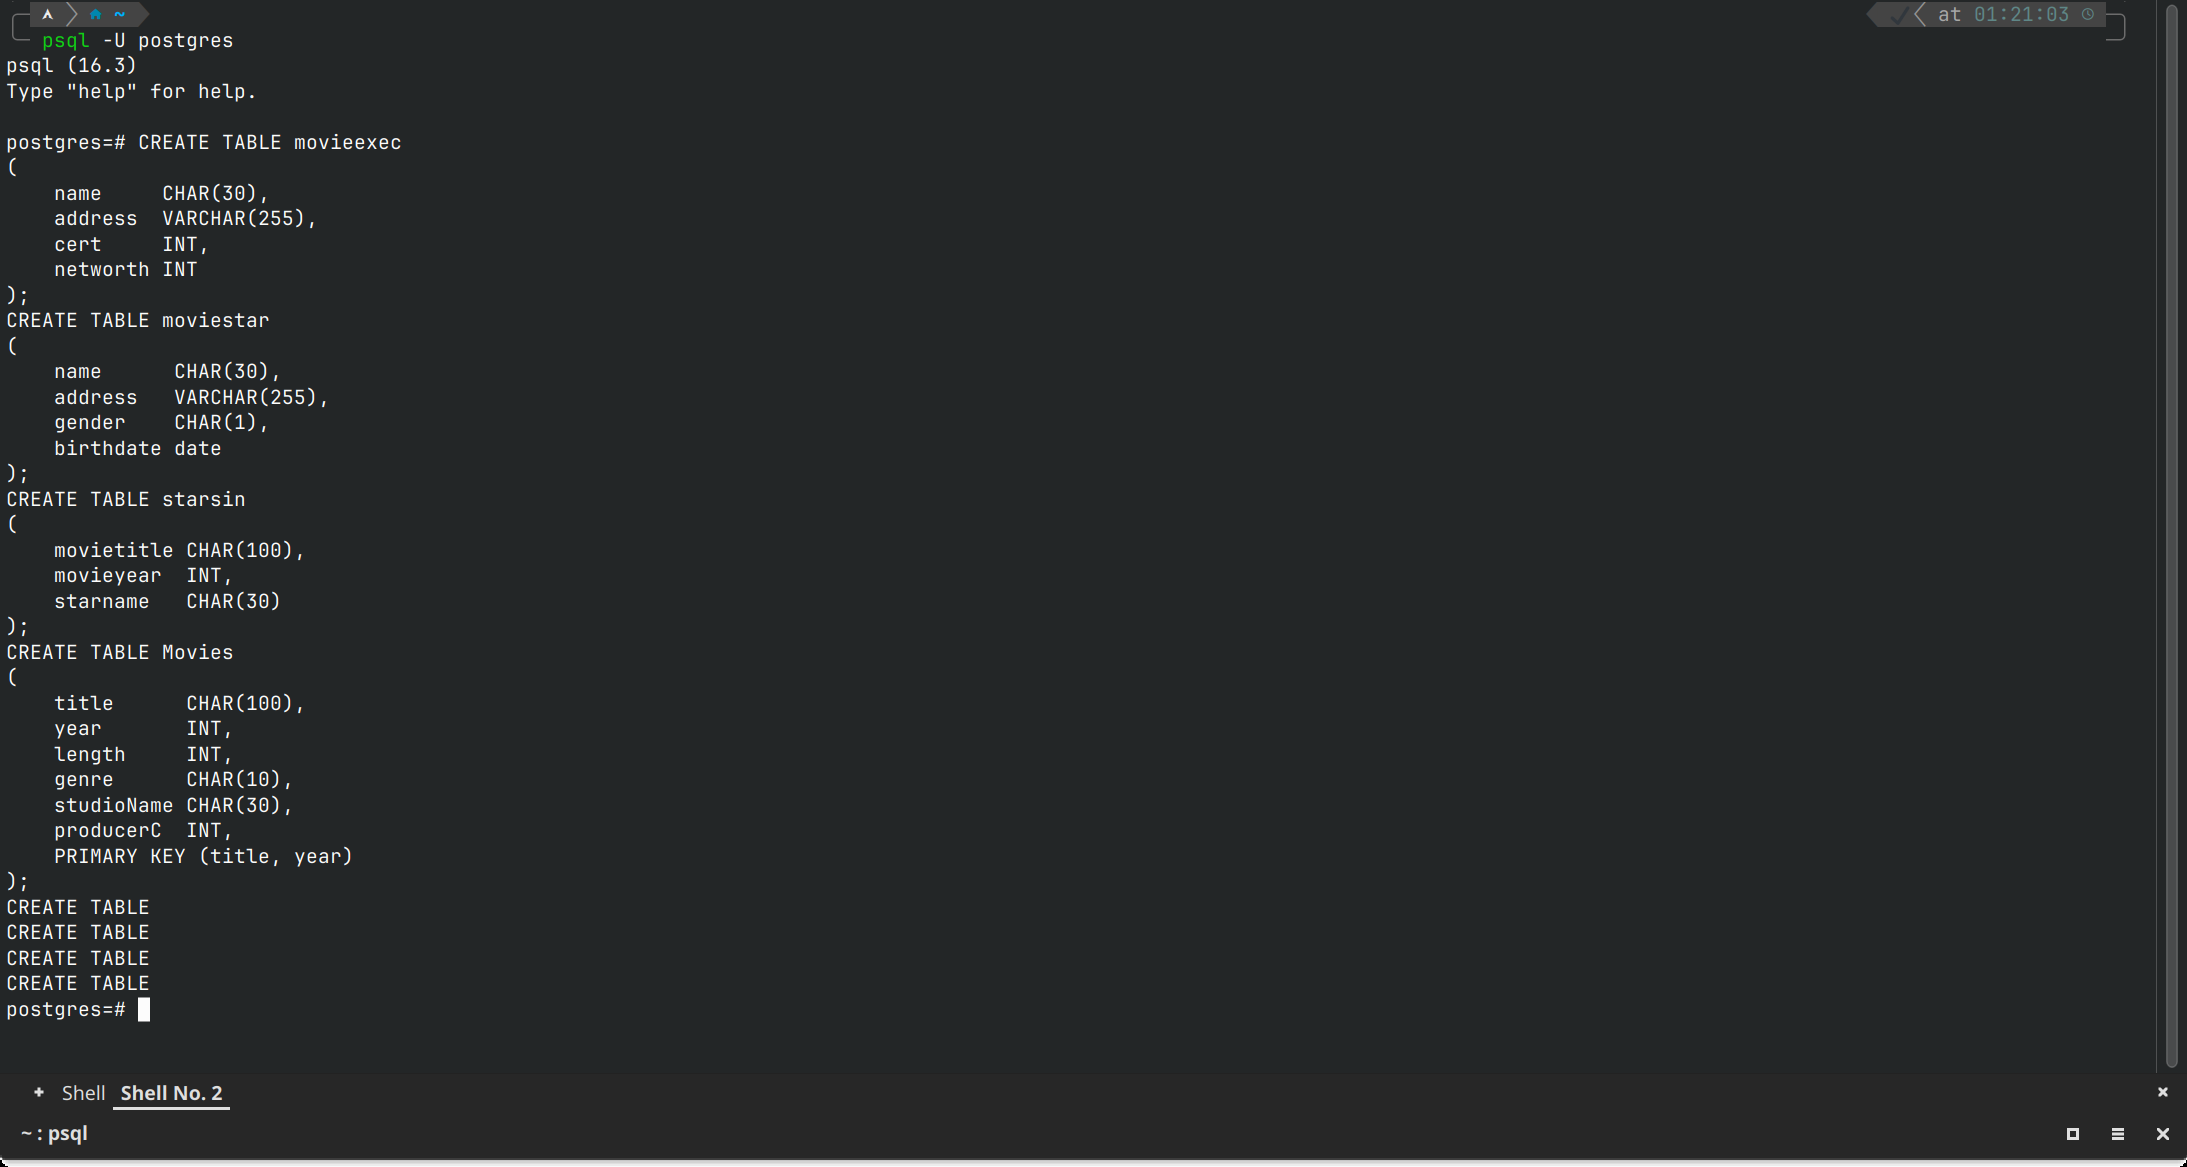
\includegraphics[width=0.8\textwidth]{hw5-1.png}
    \caption{Create Tables}
    \label{fig:create-tables}
\end{figure}

\subsubsection{Insert Sample Data \texttt{movies}}

\begin{lstlisting}[language=sql]
INSERT INTO movies VALUES ('Logan''s run', 1976, NULL, 'sciFi', 'MGM', 123);
INSERT INTO movies VALUES ('Star Wars', 1977, 124, 'sciFi', 'Fox', 555);
INSERT INTO movies VALUES ('Empire Strikes Back', 1980, 111, 'fantasy', 'Fox', 555);
INSERT INTO movies VALUES ('Star Trek', 1979, 132, 'sciFi', 'Paramount', 345);
INSERT INTO movies VALUES ('Star Trek: Nemesis', 2002, 116, 'sciFi', 'Paramount', 345);
INSERT INTO movies VALUES ('Terms of Endearment', 1983, 132, 'romance', 'MGM', 123);
INSERT INTO movies VALUES ('The Usual Suspects', 1995, 106, 'crime', 'MGM', 456);
INSERT INTO movies VALUES ('Gone With the Wind', 1938, 238, 'drama', 'MGM', 123);
INSERT INTO movies VALUES ('Wayne''s World', 1992, 95, 'comedy', 'Paramount', 123);
INSERT INTO movies VALUES ('King Kong', 2005, 187, 'drama', 'Universal', 789);
INSERT INTO movies VALUES ('King Kong', 1976, 134, 'drama', 'Paramount', 666);
INSERT INTO movies VALUES ('King Kong', 1933, 100, 'drama', 'Universal', 345);
INSERT INTO movies VALUES ('Pretty Woman', 1990, 119, 'comedy', 'Disney', 999);
\end{lstlisting}

the execution results are shown in the Fig.~\ref{fig:insert-movies}.
\begin{figure}[H]
    \centering
    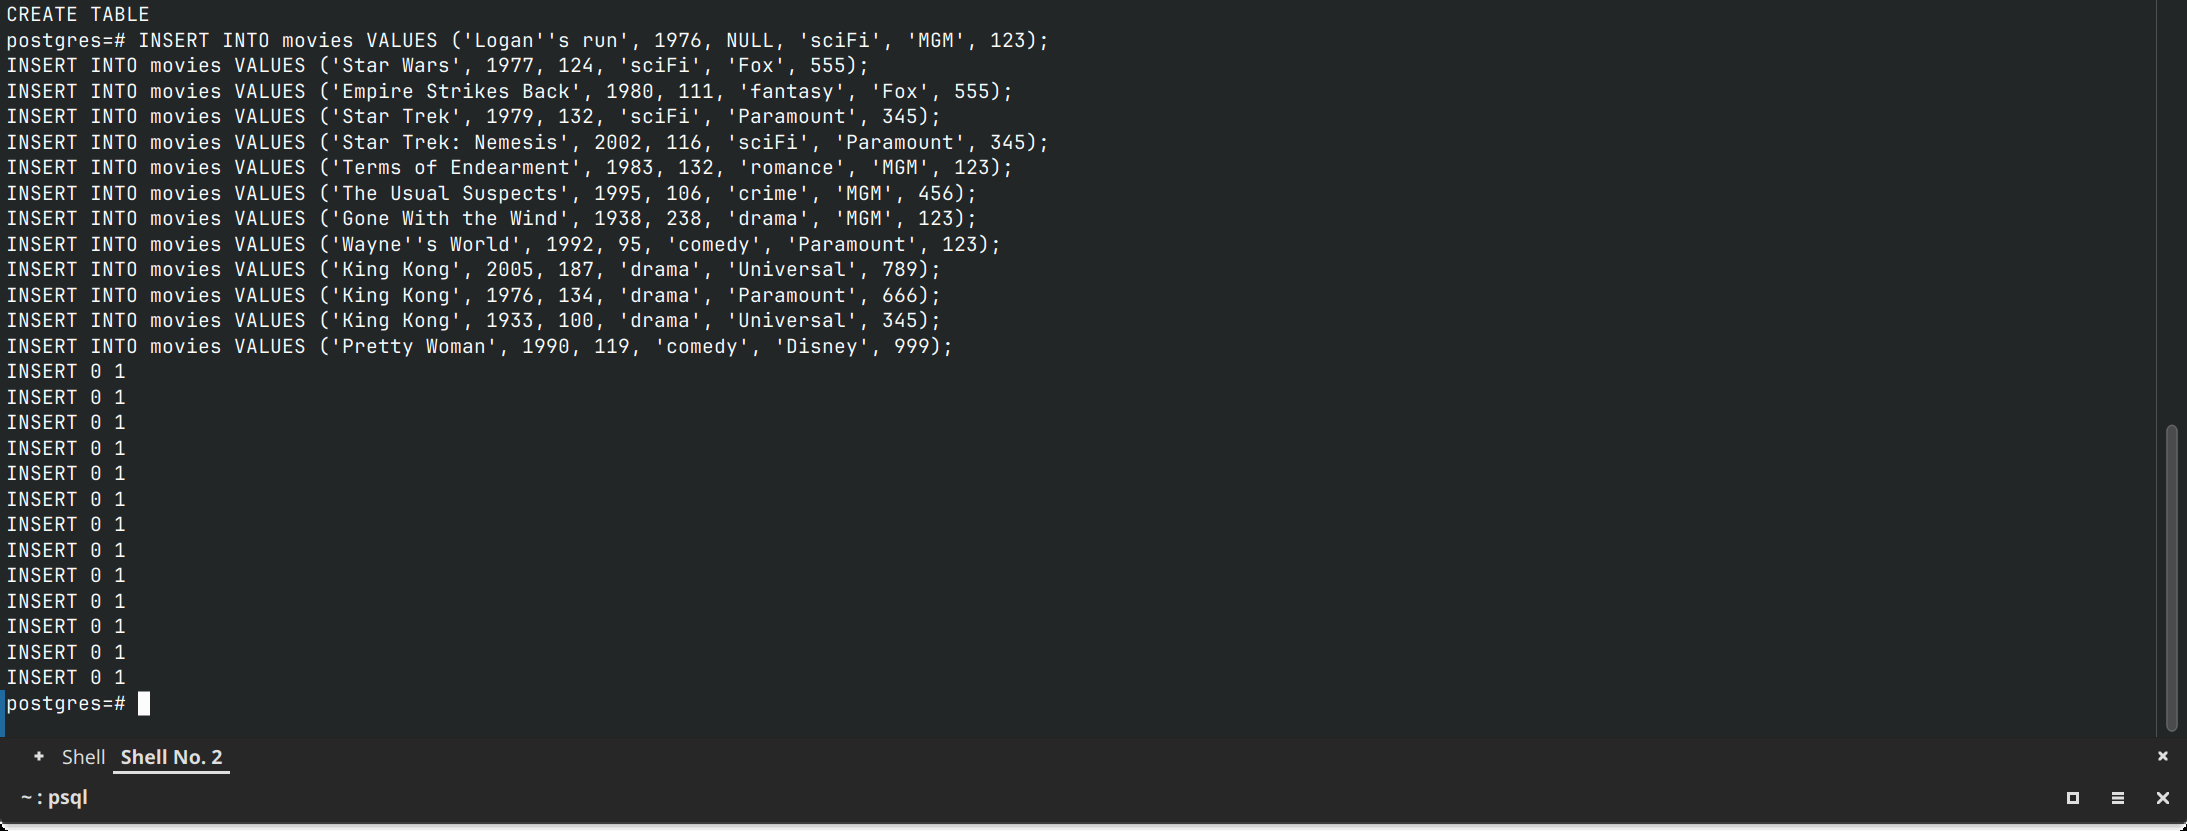
\includegraphics[width=0.8\textwidth]{hw5-2.png}
    \caption{Insert Movies}
    \label{fig:insert-movies}
\end{figure}

\subsubsection{Insert Sample Data \texttt{movieexec}}

\begin{lstlisting}[language=sql]
INSERT INTO movieexec VALUES ('George Lucas', 'Oak Rd.', 555, 200000000);
INSERT INTO movieexec VALUES ('Ted Turner', 'Turner Av.', 333, 125000000);
INSERT INTO movieexec VALUES ('Stephen Spielberg', '123 ET road', 222, 100000000);
INSERT INTO movieexec VALUES ('Merv Griffin', 'Riot Rd.', 199, 112000000);
INSERT INTO movieexec VALUES ('Calvin Coolidge', 'Fast Lane', 123, 20000000);
INSERT INTO movieexec VALUES ('Garry Marshall', 'First Street', 999, 50000000);
INSERT INTO movieexec VALUES ('J.J. Abrams', 'High Road', 345, 45000000);
INSERT INTO movieexec VALUES ('Bryan Singer', 'Downtown', 456, 70000000);
INSERT INTO movieexec VALUES ('George Roy Hill', 'Baldwin Av.', 789, 20000000);
INSERT INTO movieexec VALUES ('Dino De Laurentiis', ' Beverly Hills', 666, 120000000);
INSERT INTO movieexec VALUES ('AAA', ' Beverly Hills', 666, 120000000);
\end{lstlisting}

the execution results are shown in the Fig.~\ref{fig:insert-movieexec}.
\begin{figure}[H]
    \centering
    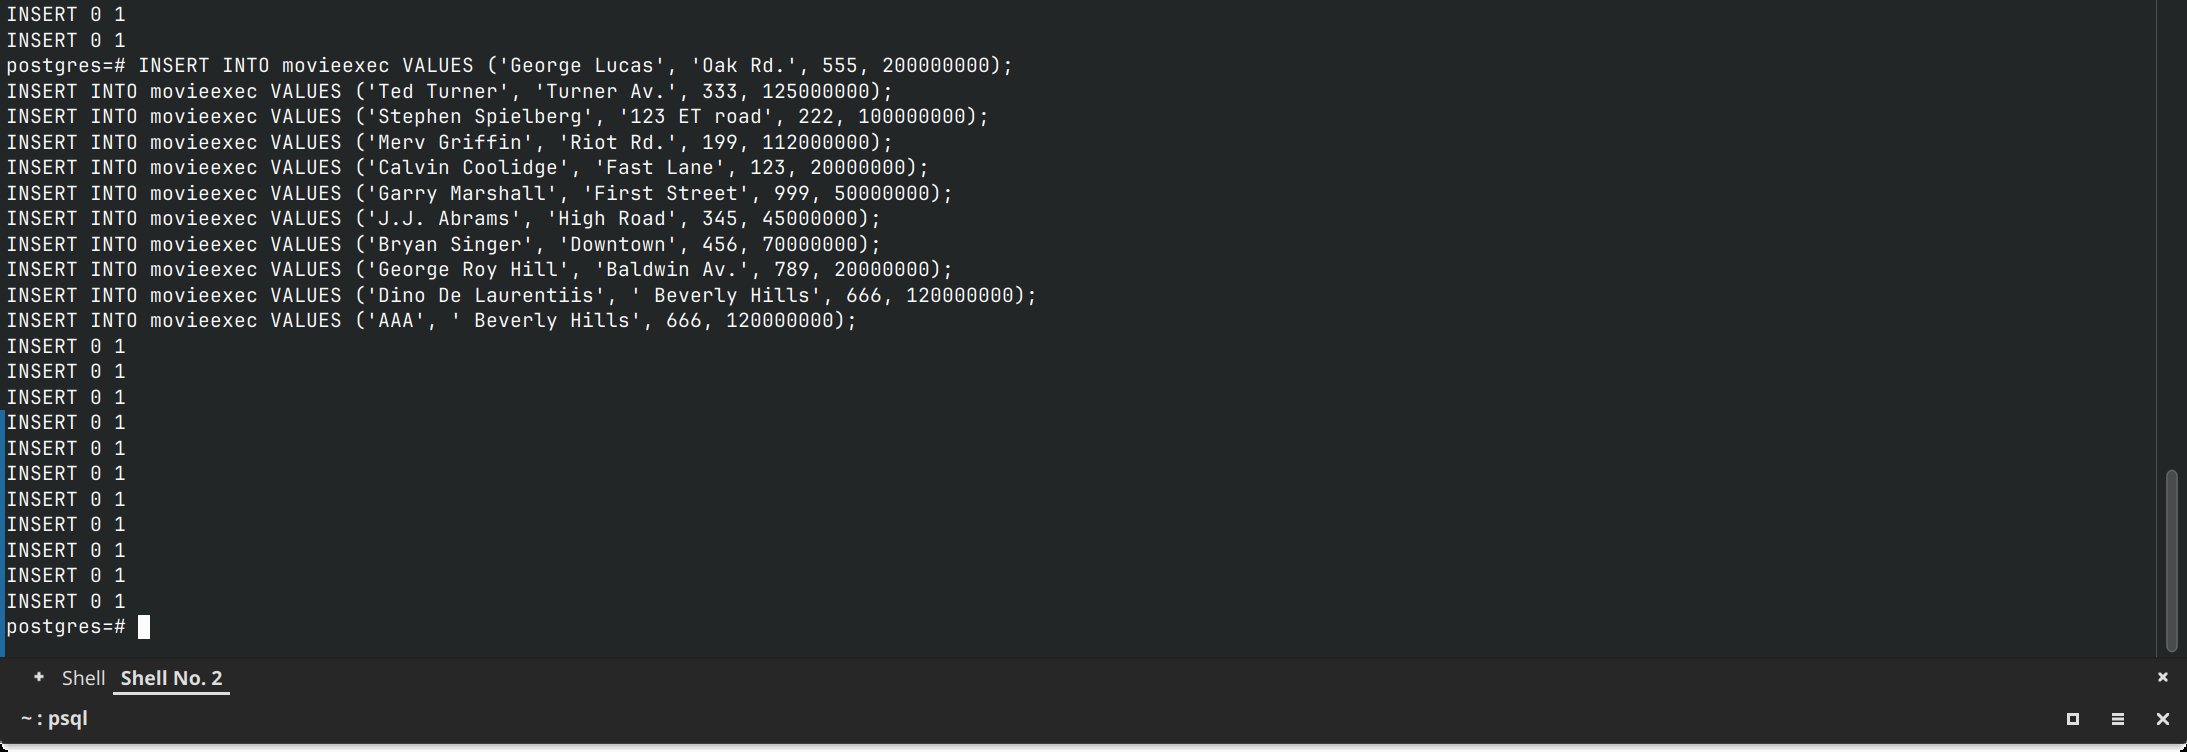
\includegraphics[width=0.8\textwidth]{hw5-3.png}
    \caption{Insert Movie Executives}
    \label{fig:insert-movieexec}
\end{figure}

\subsubsection{Insert Sample Data \texttt{moviestar}}

\begin{lstlisting}[language=sql]
INSERT INTO moviestar VALUES ('Jane Fonda', 'Turner Av.', 'F', '1977-07-07');
INSERT INTO moviestar VALUES ('Alec Baldwin', 'Baldwin Av.', 'M', '1977-06-07');
INSERT INTO moviestar VALUES ('Kim Basinger', 'Baldwin Av.', 'F', '1979-05-07');
INSERT INTO moviestar VALUES ('Harrison Ford', 'Beverly Hills', 'M', '1977-07-07');
INSERT INTO moviestar VALUES ('Carrie Fisher', '123 Maple St.', 'F', '1999-09-09');
INSERT INTO moviestar VALUES ('Mark Hamill', '456 Oak Rd.', 'M', '1988-08-08');
INSERT INTO moviestar VALUES ('Debra Winger', 'A way', 'F', '1978-05-06');
INSERT INTO moviestar VALUES ('Jack Nicholson', 'X path', 'M', '1949-05-05');
INSERT INTO moviestar VALUES ('Kevin Spacey', 'New York Av.', 'F', '1937-12-21');
INSERT INTO moviestar VALUES ('AAA', 'New York Av.', 'F', '1937-12-21');
\end{lstlisting}

the execution results are shown in the Fig.~\ref{fig:insert-moviestar}.
\begin{figure}[H]
    \centering
    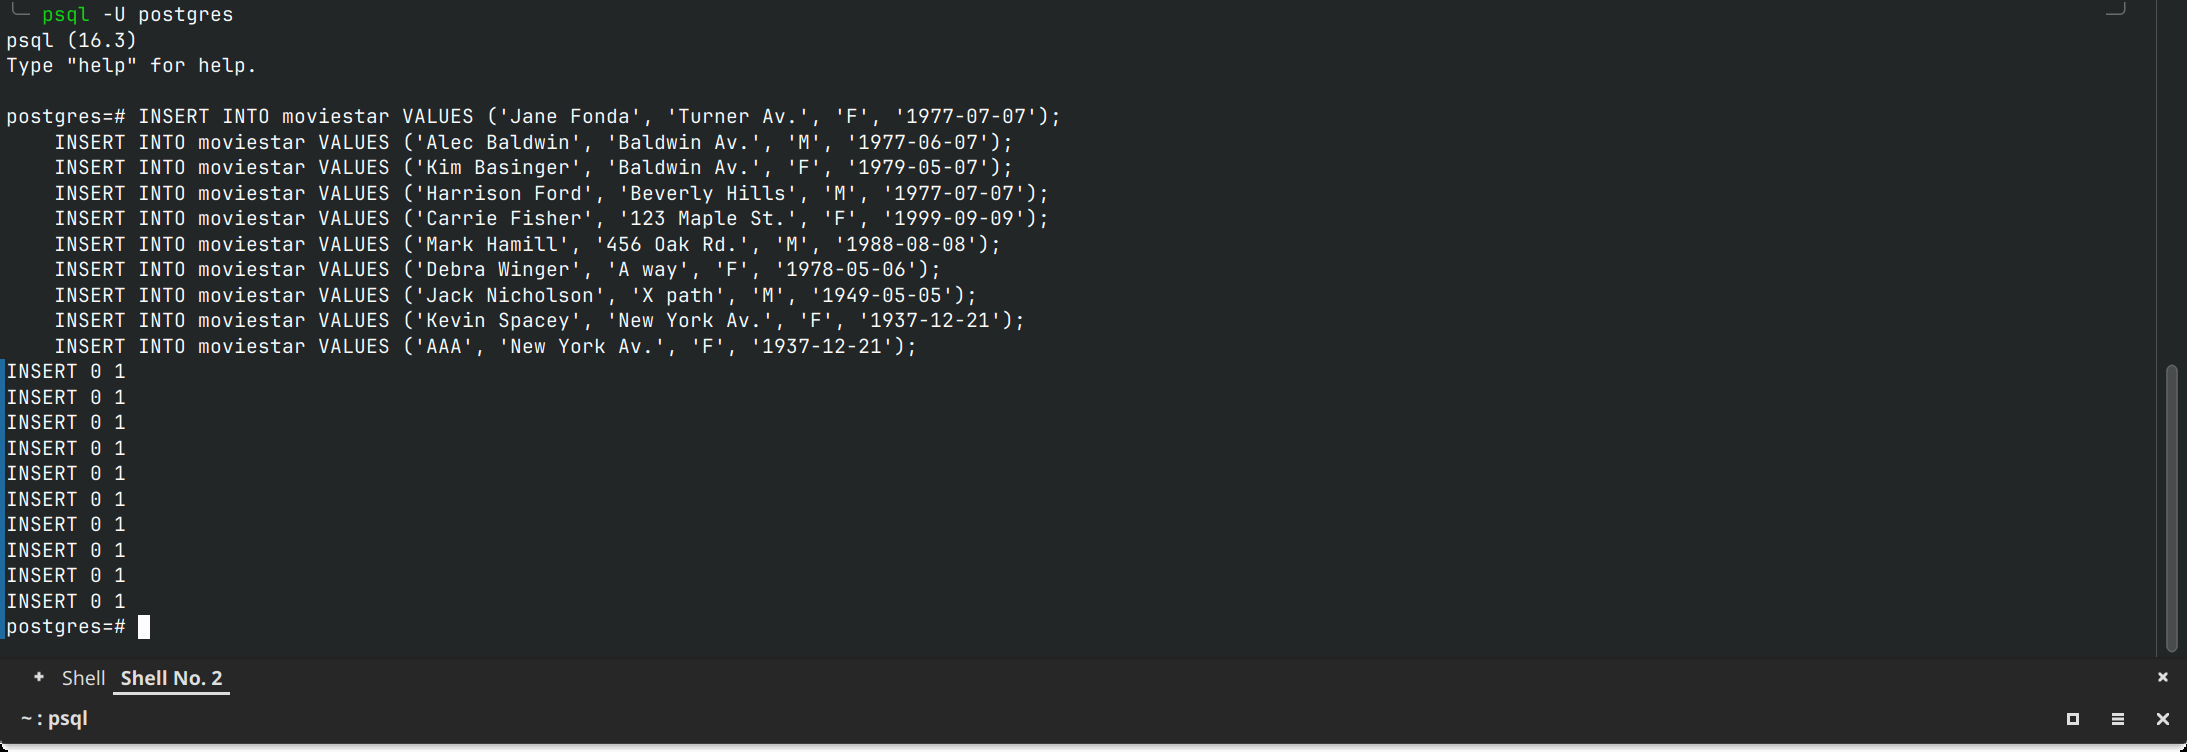
\includegraphics[width=0.8\textwidth]{hw5-4.png}
    \caption{Insert Movie Stars}
    \label{fig:insert-moviestar}
\end{figure}


\subsubsection{Insert Sample Data \texttt{starsin}}

\begin{lstlisting}[language=sql]
INSERT INTO starsin VALUES ('Star Wars', 1977, 'Carrie Fisher');
INSERT INTO starsin VALUES ('Star Wars', 1977, 'Mark Hamill');
INSERT INTO starsin VALUES ('Star Wars', 1977, 'Harrison Ford');
INSERT INTO starsin VALUES ('Empire Strikes Back', 1980, 'Harrison Ford');
INSERT INTO starsin VALUES ('The Usual Suspects', 1995, 'Kevin Spacey');
INSERT INTO starsin VALUES ('Terms of Endearment', 1983, 'Debra Winger');
INSERT INTO starsin VALUES ('Terms of Endearment', 1983, 'Jack Nicholson');
\end{lstlisting}

the execution results are shown in the Fig.~\ref{fig:insert-starsin}.

\begin{figure}[H]
    \centering
    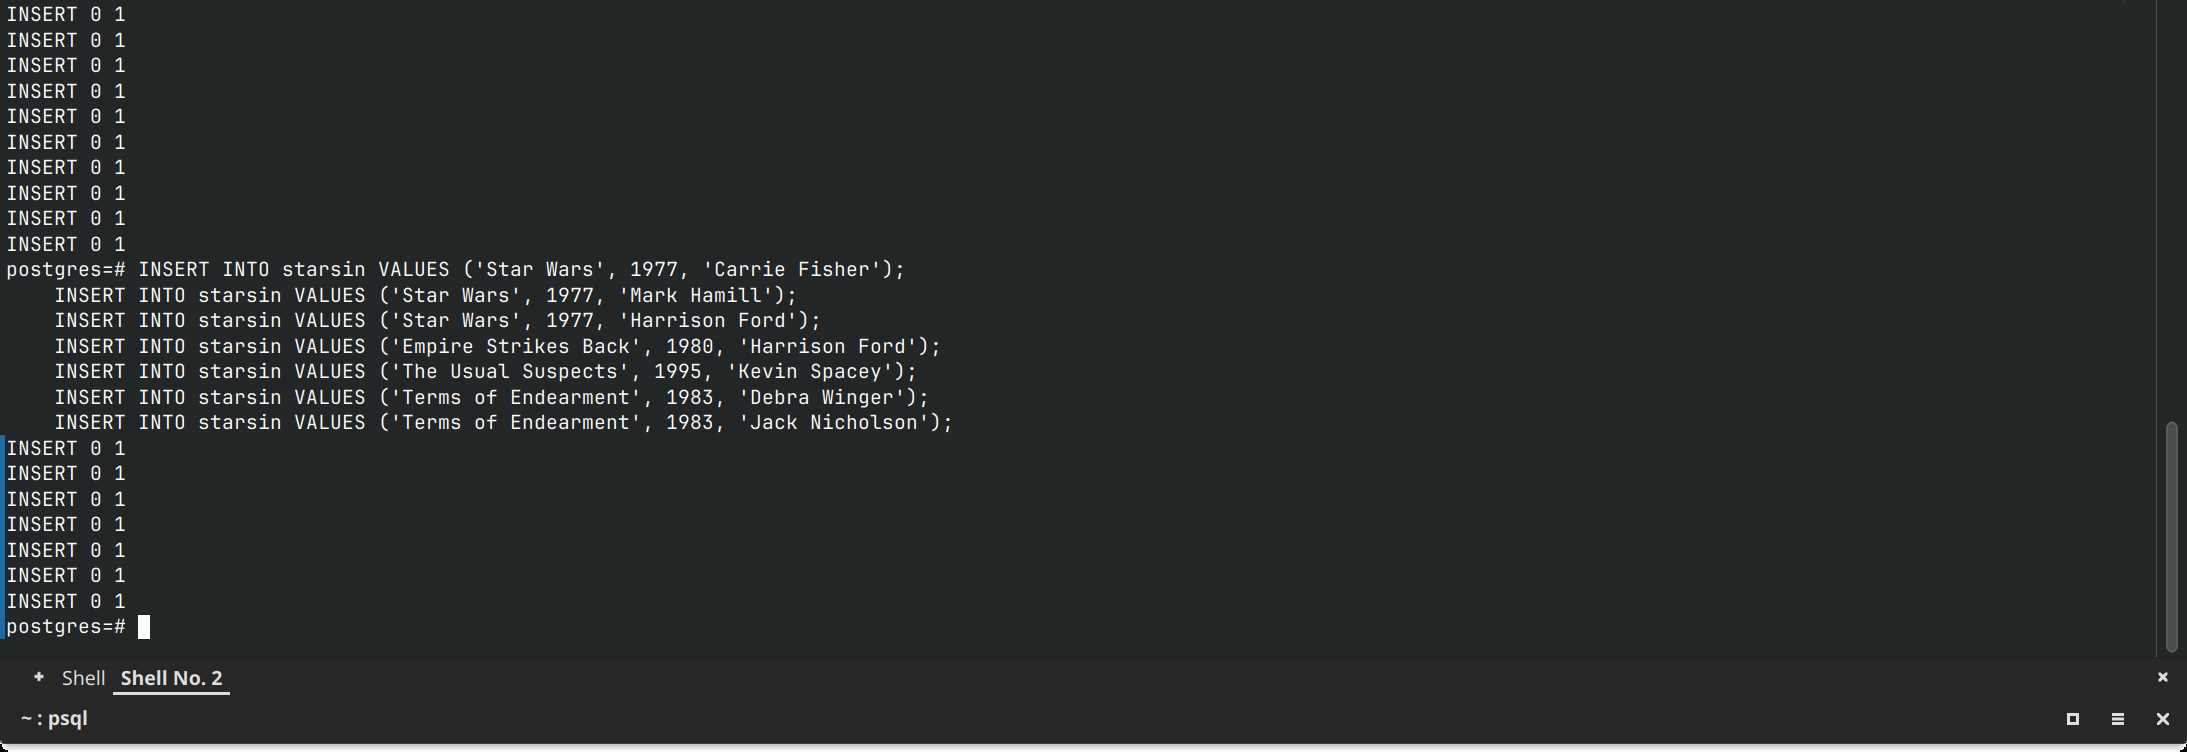
\includegraphics[width=0.8\textwidth]{hw5-5.png}
    \caption{Insert Stars In}
    \label{fig:insert-starsin}
\end{figure}

\subsection{Queries}

\subsubsection{subquery}

\begin{lstlisting}[language=sql]
SELECT name
FROM MovieExec
WHERE cert =
        (SELECT producerC
        FROM Movies
        WHERE title = 'Star Wars');

SELECT name
FROM MovieExec
WHERE cert =
        (SELECT *
        FROM Movies
        WHERE title = 'Star Wars');
\end{lstlisting}

the execution results are shown in the Fig.~\ref{fig:subquery}.
\begin{figure}[H]
    \centering
    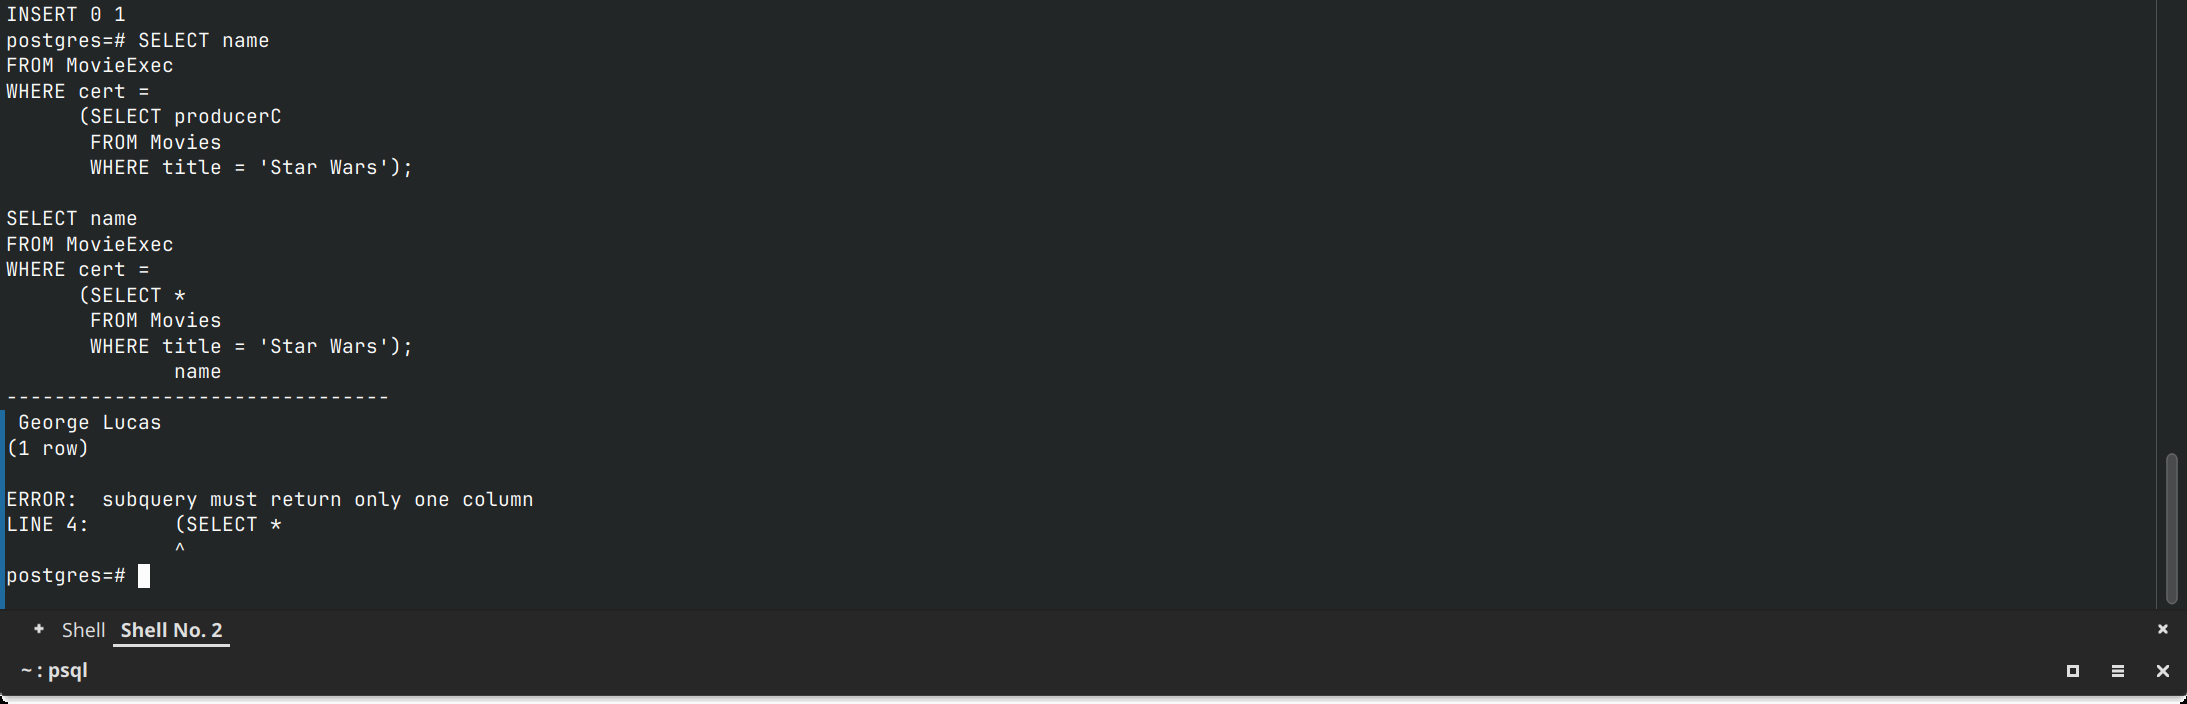
\includegraphics[width=0.8\textwidth]{hw5-6.png}
    \caption{Subquery}
    \label{fig:subquery}
\end{figure}

\subsubsection{conditions Involve Relations}

\begin{lstlisting}[language=sql]
SELECT name
FROM MovieExec
WHERE Exists
            (SELECT producerC
            FROM Movies
            WHERE title like 'Star%');
SELECT *
FROM MovieExec
WHERE cert in
        (SELECT producerC FROM Movies);

SELECT *
FROM movies
WHERE length > all (SELECT length FROM movies);

SELECT *
FROM movies
WHERE length<any(SELECT length FROM movies);
\end{lstlisting}

the execution results are shown in the Fig.~\ref{fig:conditions-involve-relations-1}.

\begin{figure}[H]
    \centering
    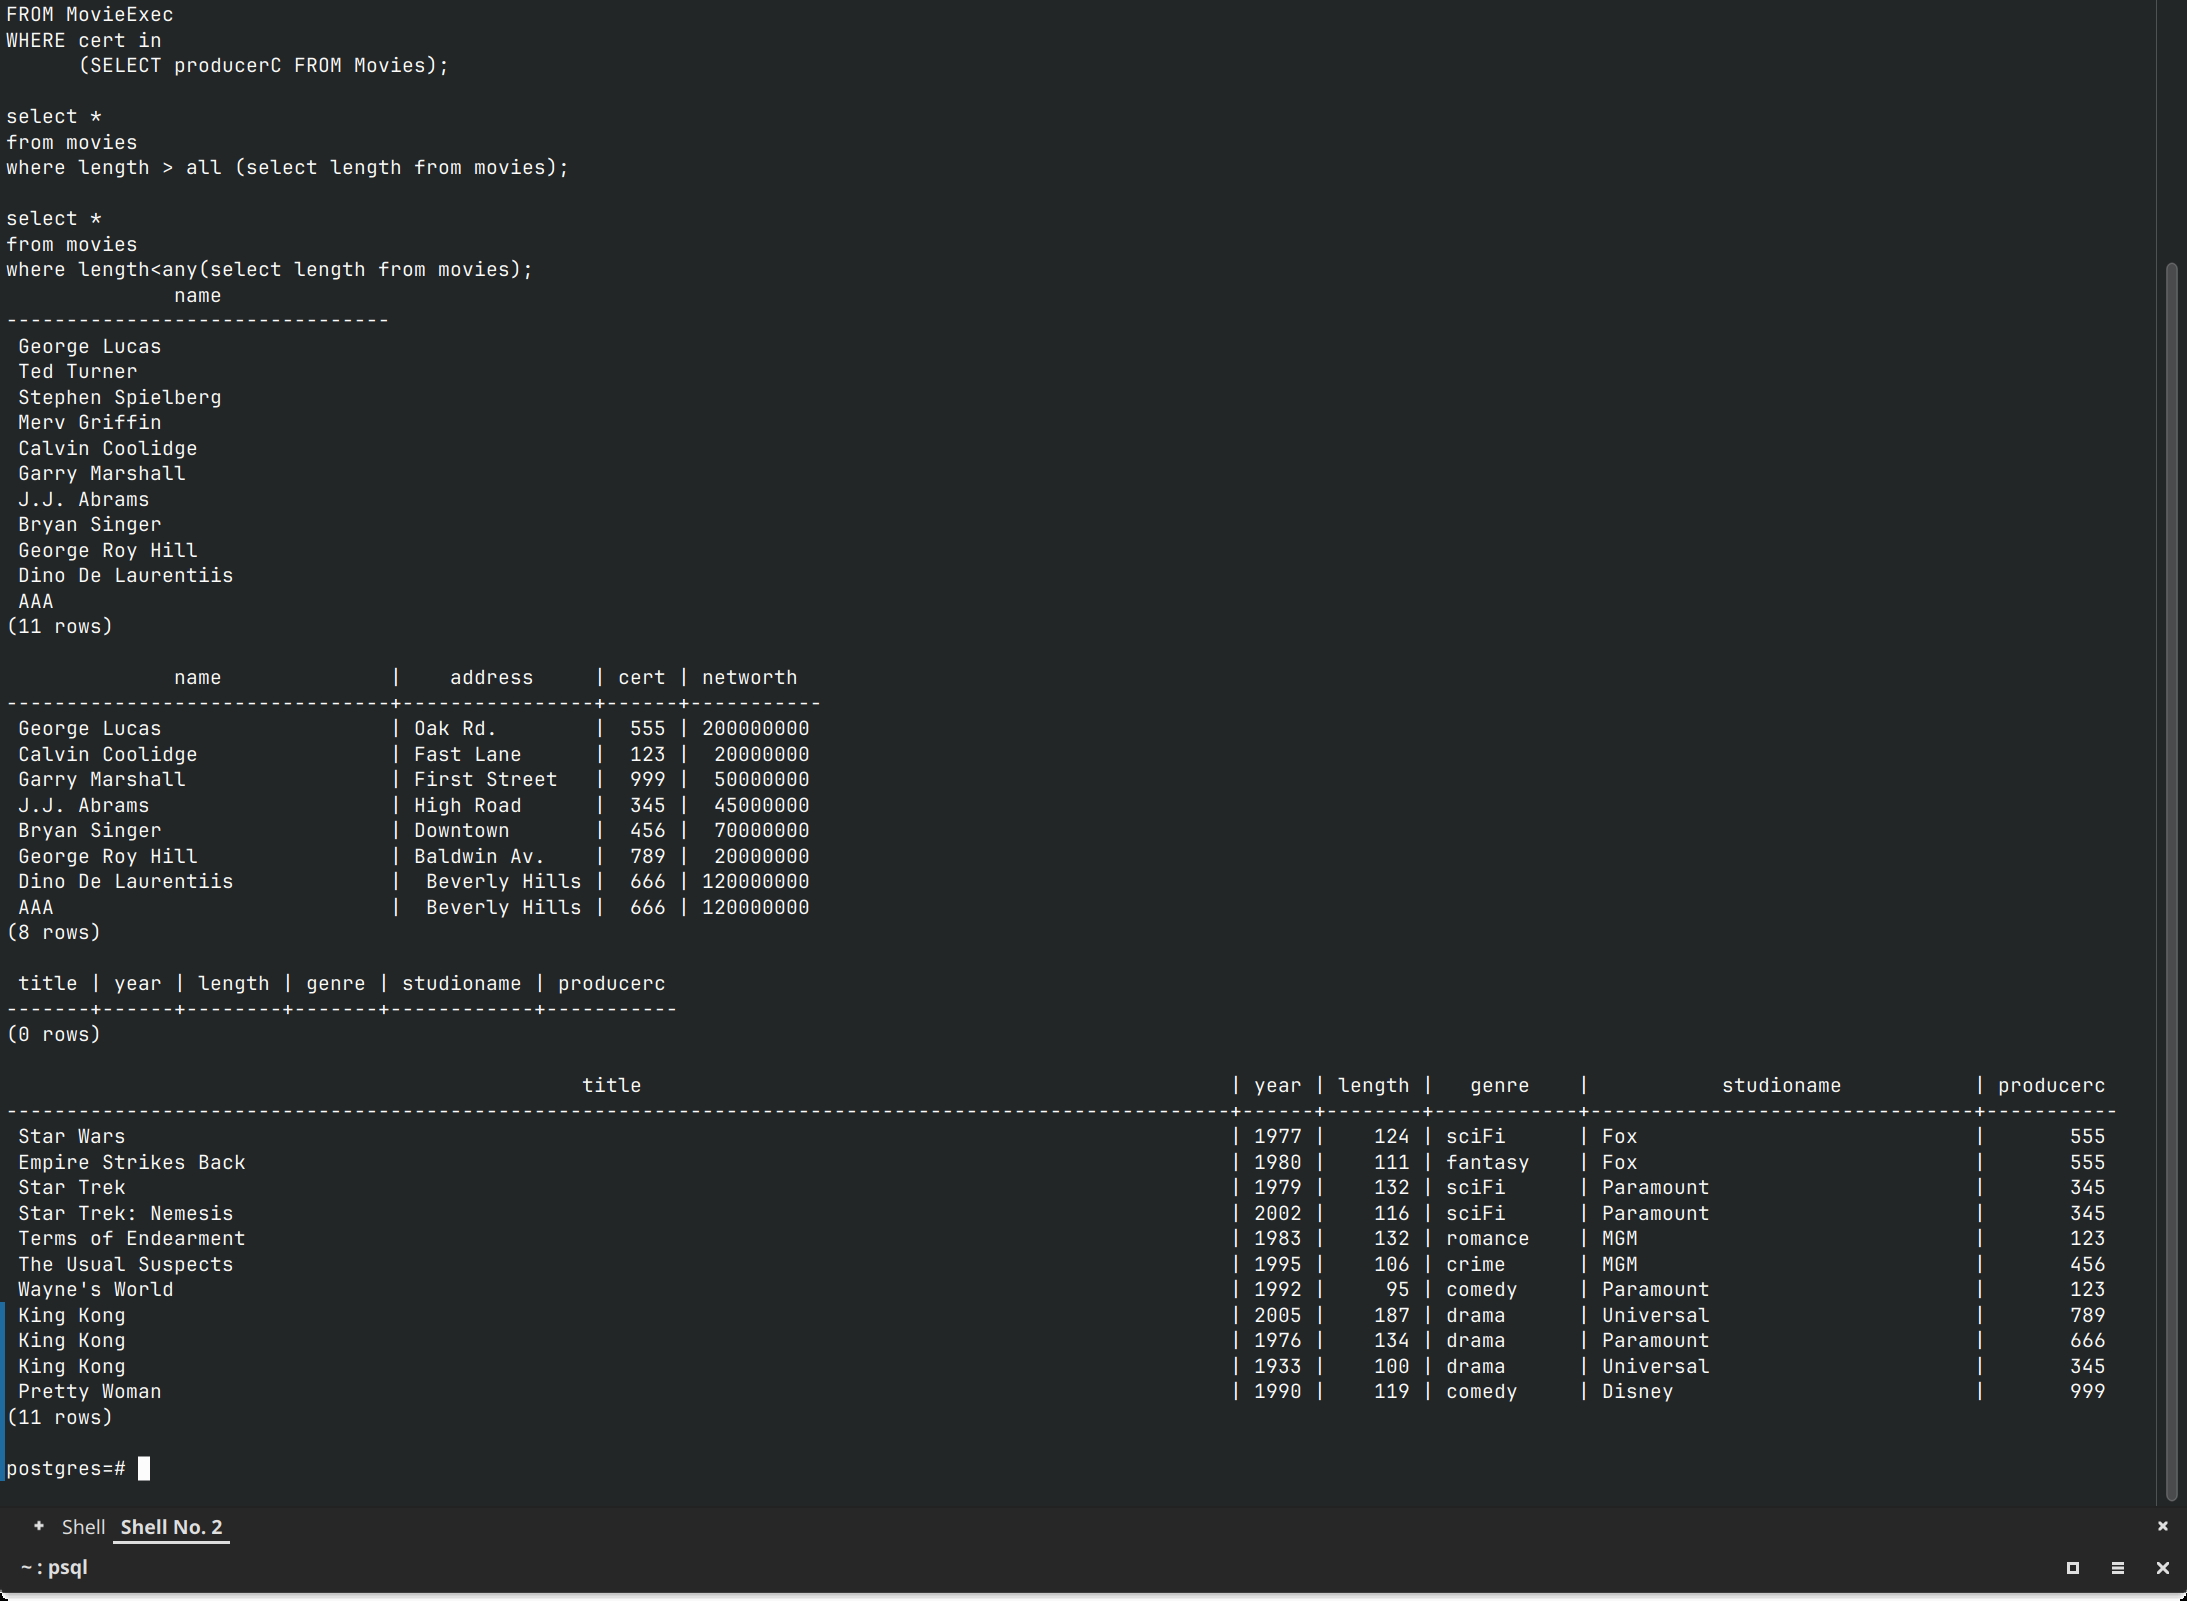
\includegraphics[width=0.8\textwidth]{hw5-7.png}
    \caption{Conditions Involve Relations}
    \label{fig:conditions-involve-relations-1}
\end{figure}

\begin{lstlisting}[language=sql]
SELECT name
FROM MovieExec
WHERE cert IN
      (SELECT producerC
       FROM Movies
       WHERE (title, year) IN
             (SELECT movieTitle, movieYear
              FROM StarsIn
              WHERE starName = 'Harrison Ford'));
\end{lstlisting}

the execution results are shown in the Fig.~\ref{fig:conditions-involve-relations-2}.

\begin{figure}[H]
    \centering
    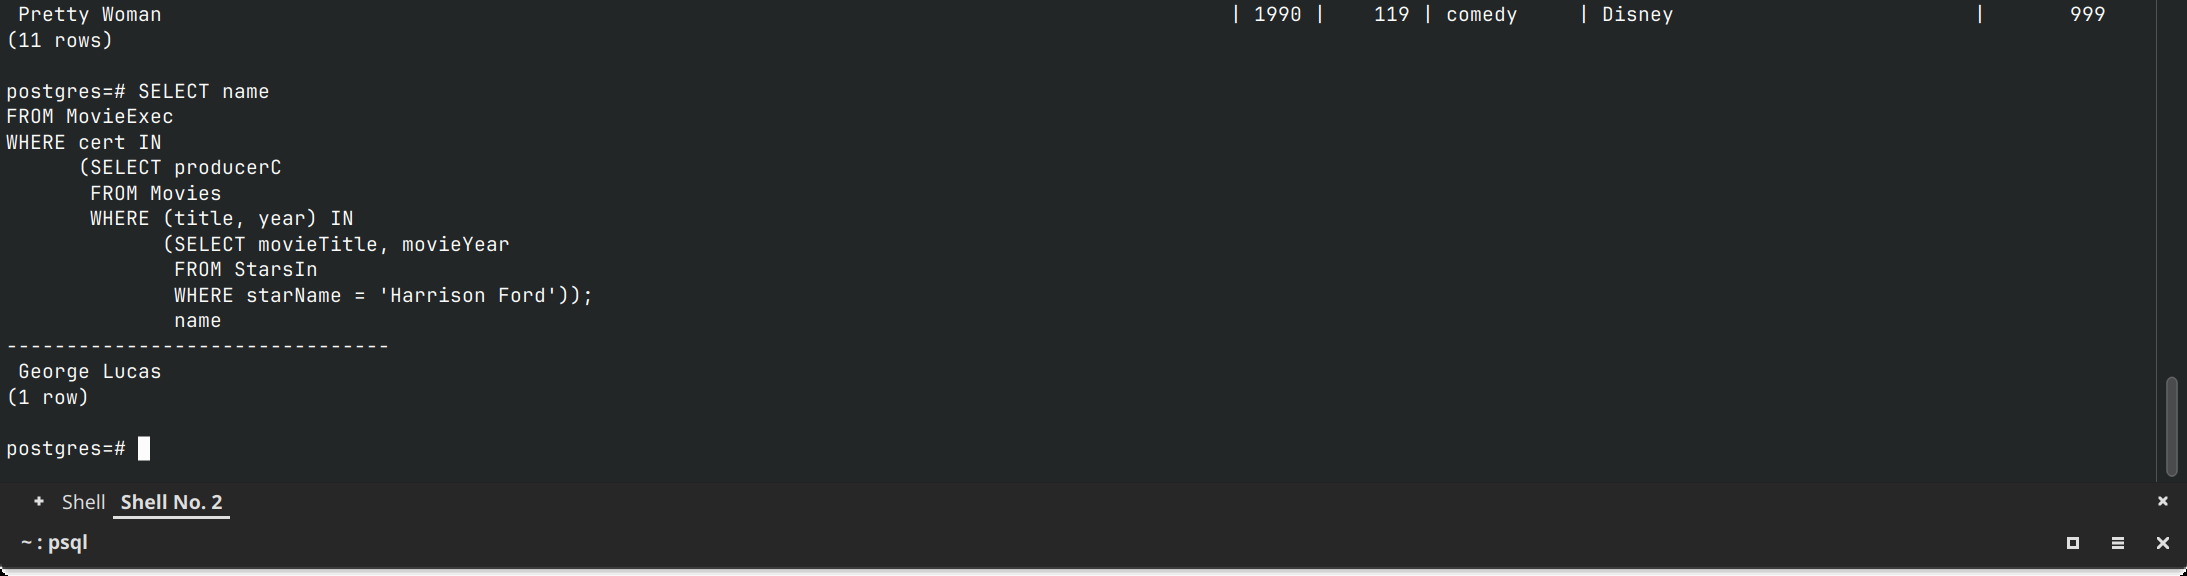
\includegraphics[width=0.8\textwidth]{hw5-8.png}
    \caption{Conditions Involve Relations}
    \label{fig:conditions-involve-relations-2}
\end{figure}

\subsubsection{Correlated Subqueries}

\begin{lstlisting}[language=sql]
SELECT *
FROM Movies Old
WHERE year < ANY
      (SELECT year
       FROM Movies
       WHERE title = Old.title);

SELECT *
FROM MovieExec,
     (SELECT producerC
      FROM Movies,
           StarsIn
      WHERE title = movieTitle
        AND year = movieYear
        AND starName = 'Harrison Ford') Prod
WHERE cert = Prod.producerC;
\end{lstlisting}

the execution results are shown in the Fig.~\ref{fig:correlated-subqueries}.

\begin{figure}[H]
    \centering
    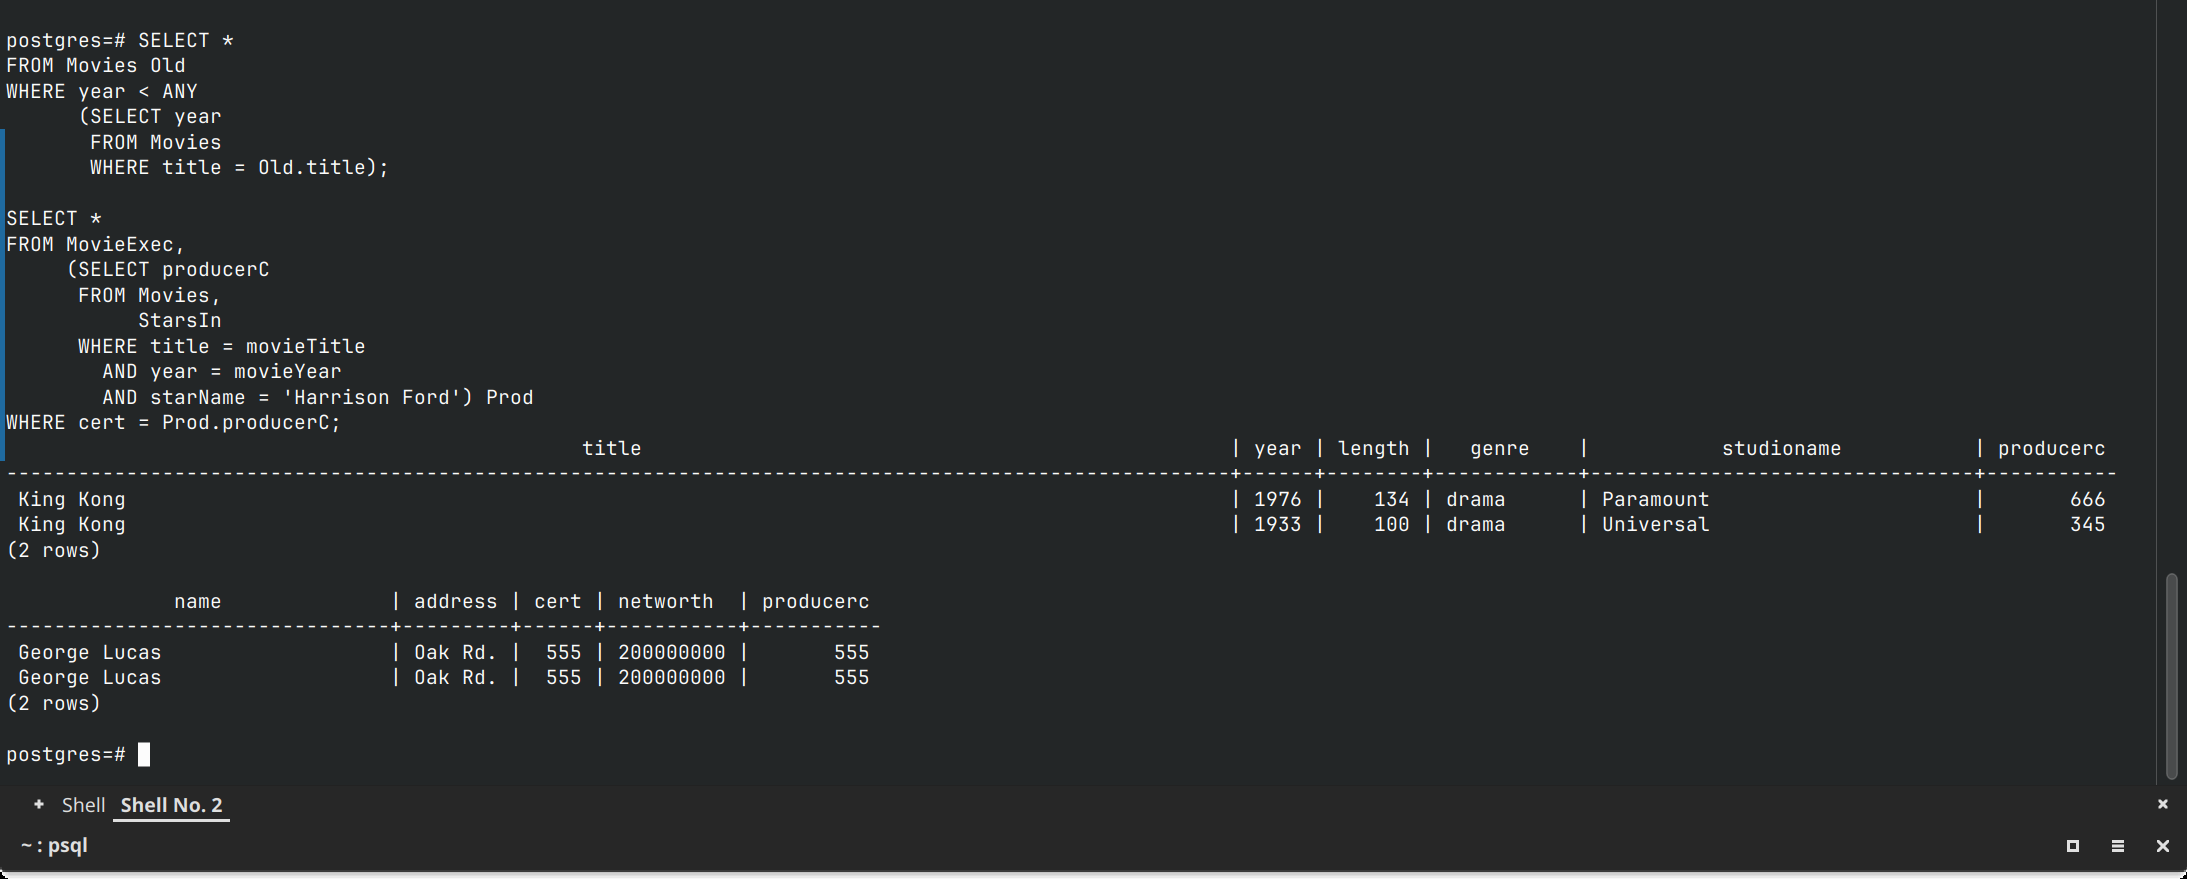
\includegraphics[width=0.8\textwidth]{hw5-9.png}
    \caption{Correlated Subqueries}
    \label{fig:correlated-subqueries}
\end{figure}

\subsubsection{Join Expression}

\begin{lstlisting}[language=sql]
SELECT *
FROM Movies
            JOIN StarsIn ON
    title = movieTitle AND year = movieYear;

SELECT *
FROM Movies
            JOIN StarsIn ON
    title = movieTitle AND year = movieYear
        AND starName = 'Harrison Ford';
\end{lstlisting}

the execution results are shown in the Fig.~\ref{fig:join-expression}.
\begin{figure}[H]
    \centering
    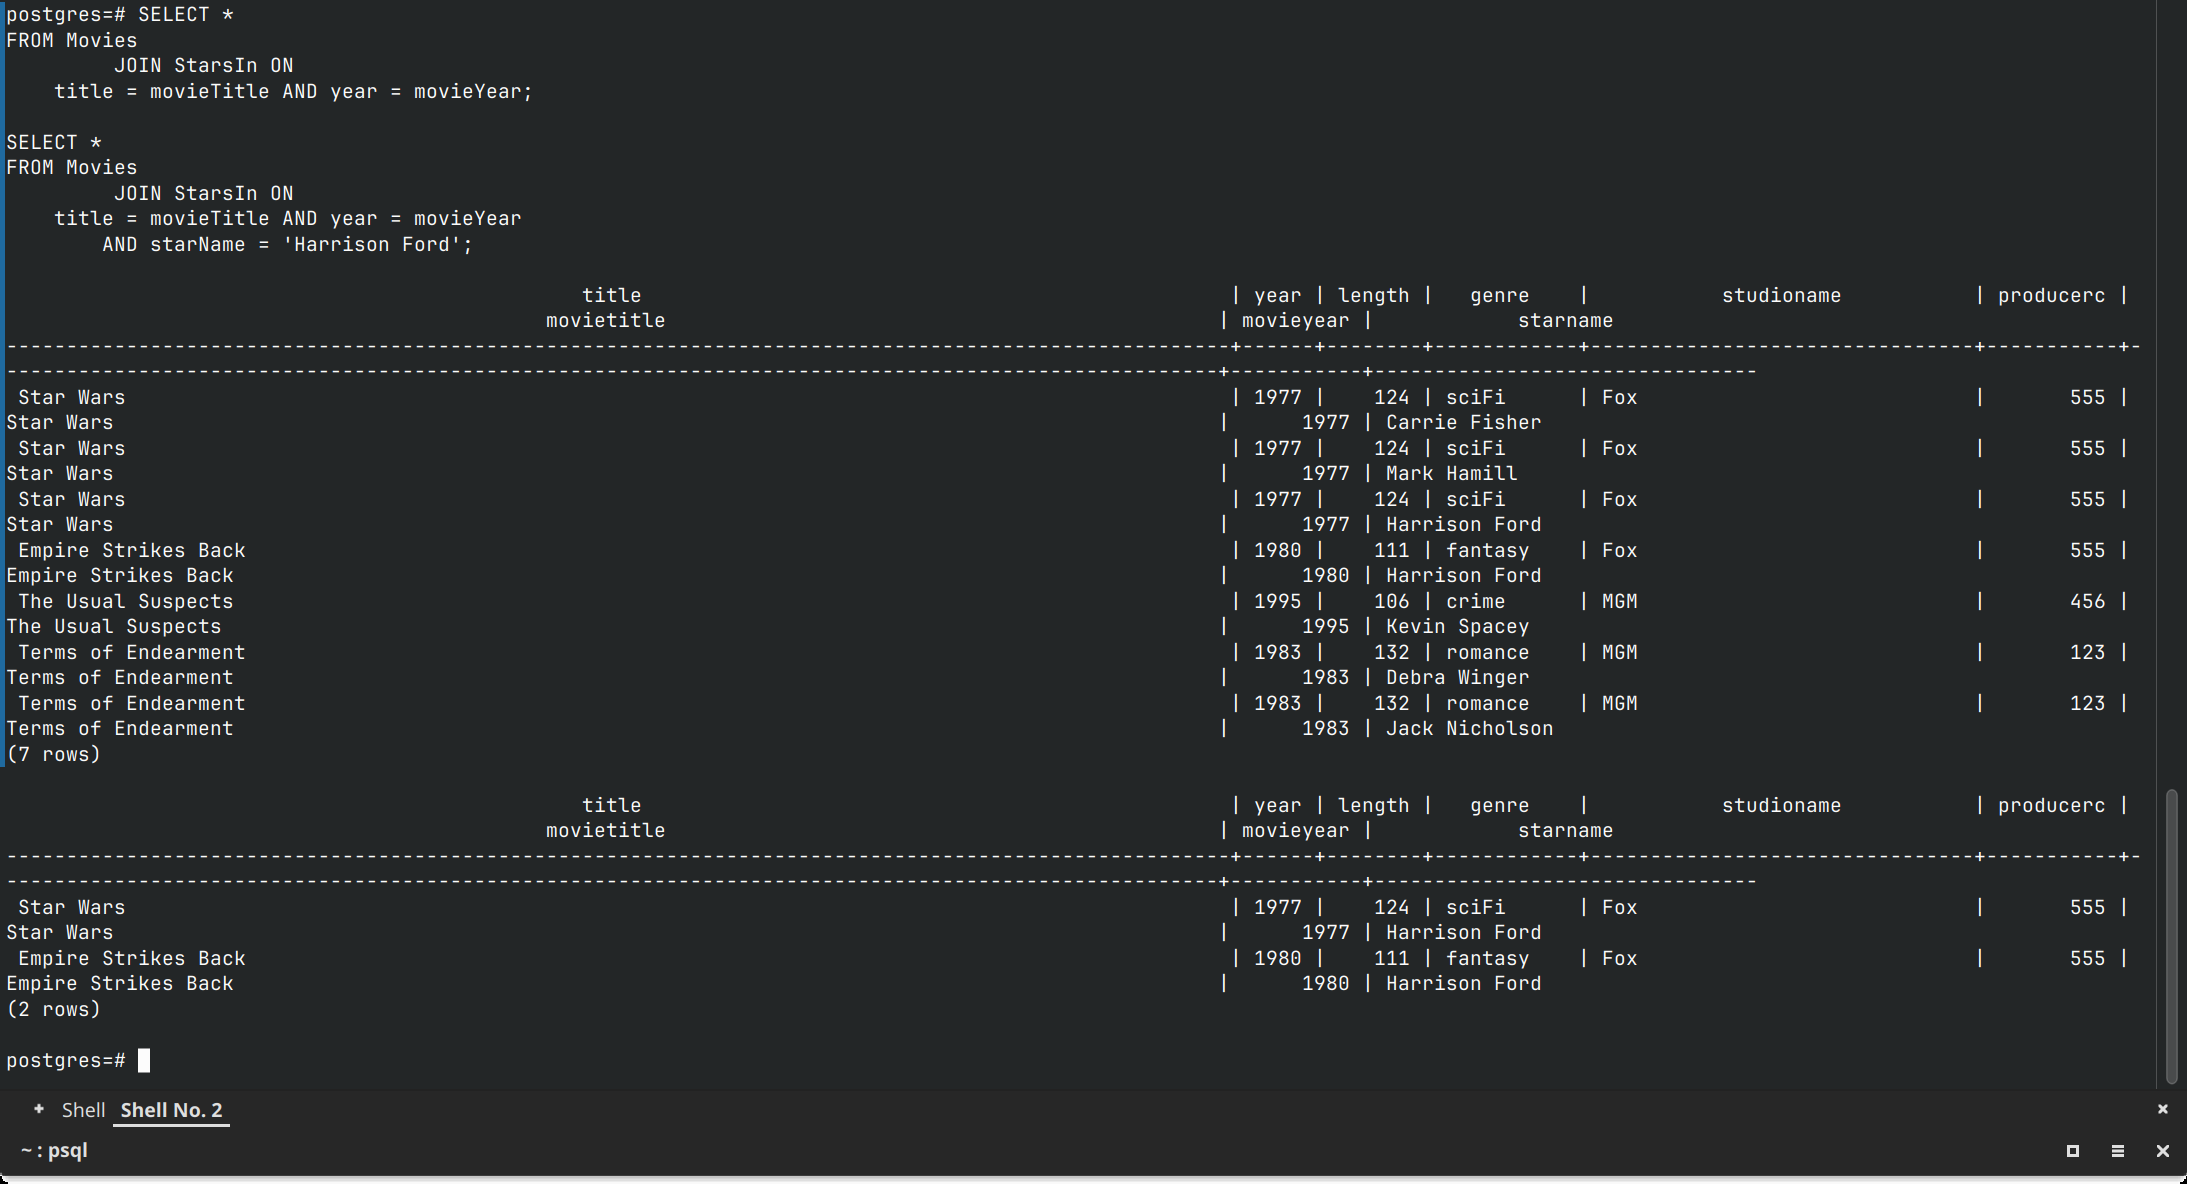
\includegraphics[width=0.8\textwidth]{hw5-10.png}
    \caption{Join Expression}
    \label{fig:join-expression}
\end{figure}

\subsubsection{Join Types}

\begin{lstlisting}[language=sql]
SELECT *
from MovieStar
            NATURAL JOIN MovieExec;

SELECT *
From Movies
            NATURAL full outer JOIN StarsIn;

SELECT *
From Movies
            NATURAL left outer JOIN StarsIn;

SELECT *
From Movies
            NATURAL right outer JOIN StarsIn;
\end{lstlisting}

the execution results are shown in the Fig.~\ref{fig:join-types-1}-\ref{fig:join-types-4}.
\begin{figure}[H]
    \centering
    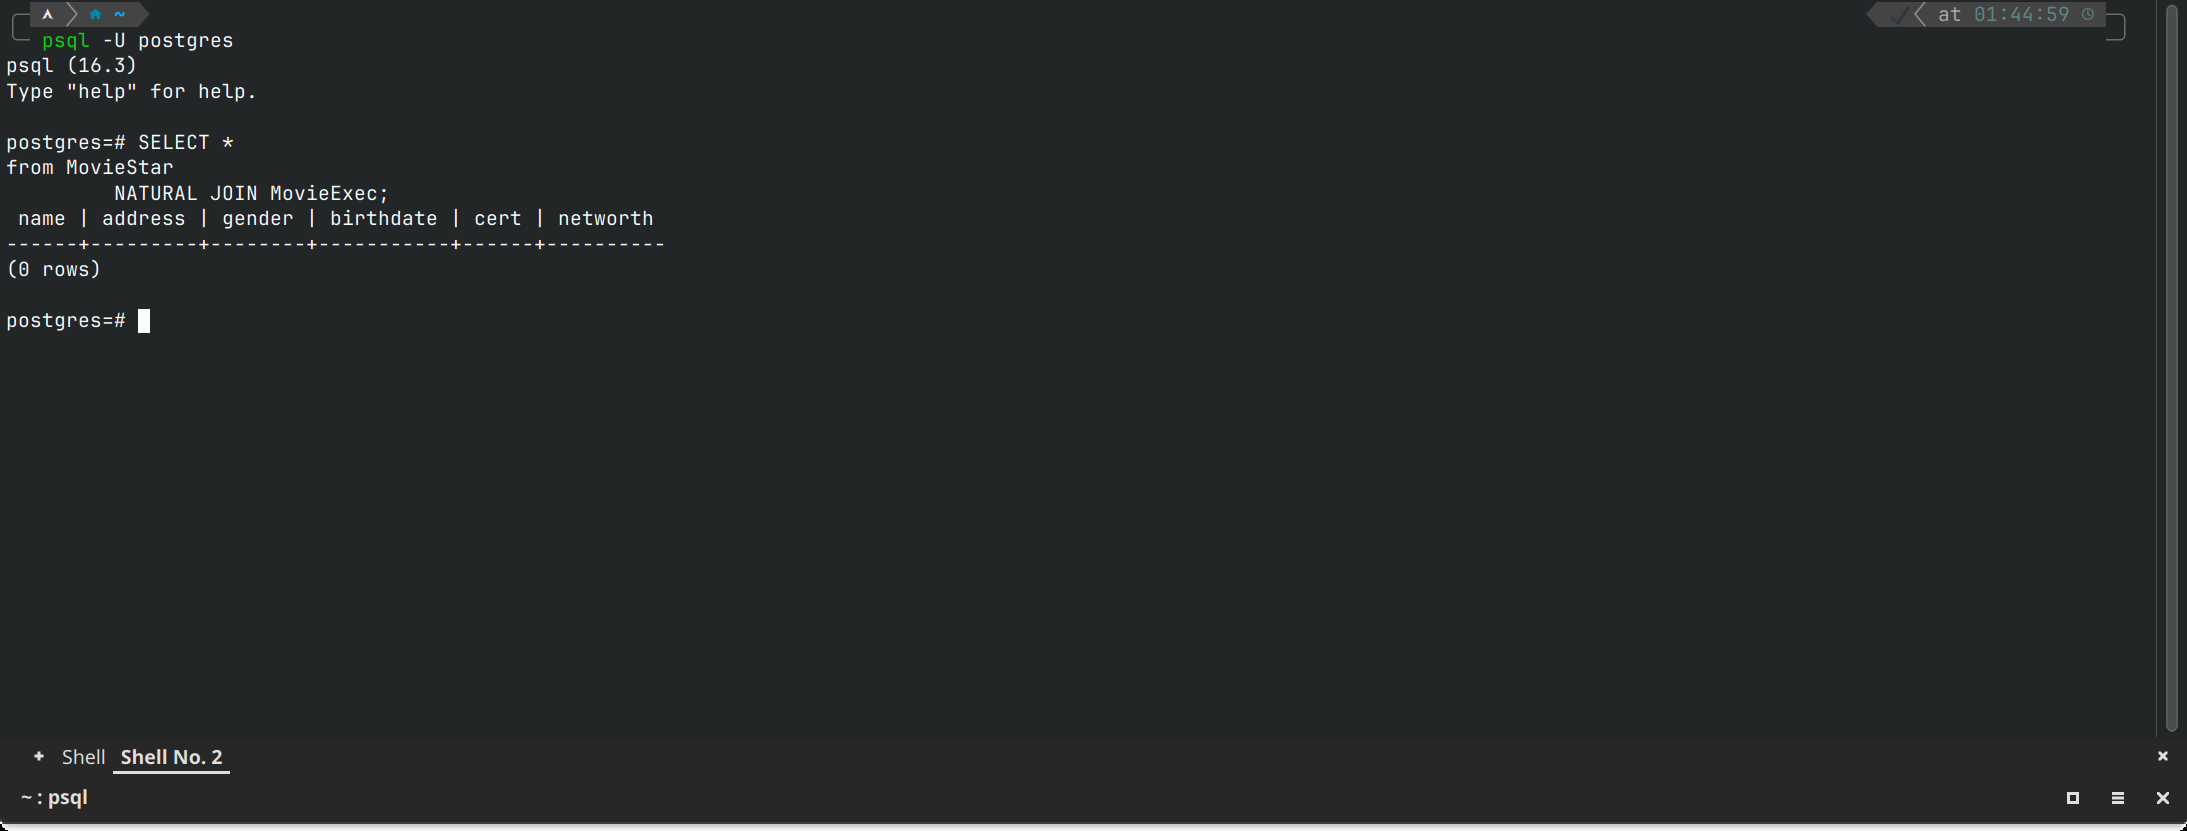
\includegraphics[width=0.8\textwidth]{hw5-11.png}
    \caption{Join Types}
    \label{fig:join-types-1}
\end{figure}

\begin{figure}[H]
    \centering
    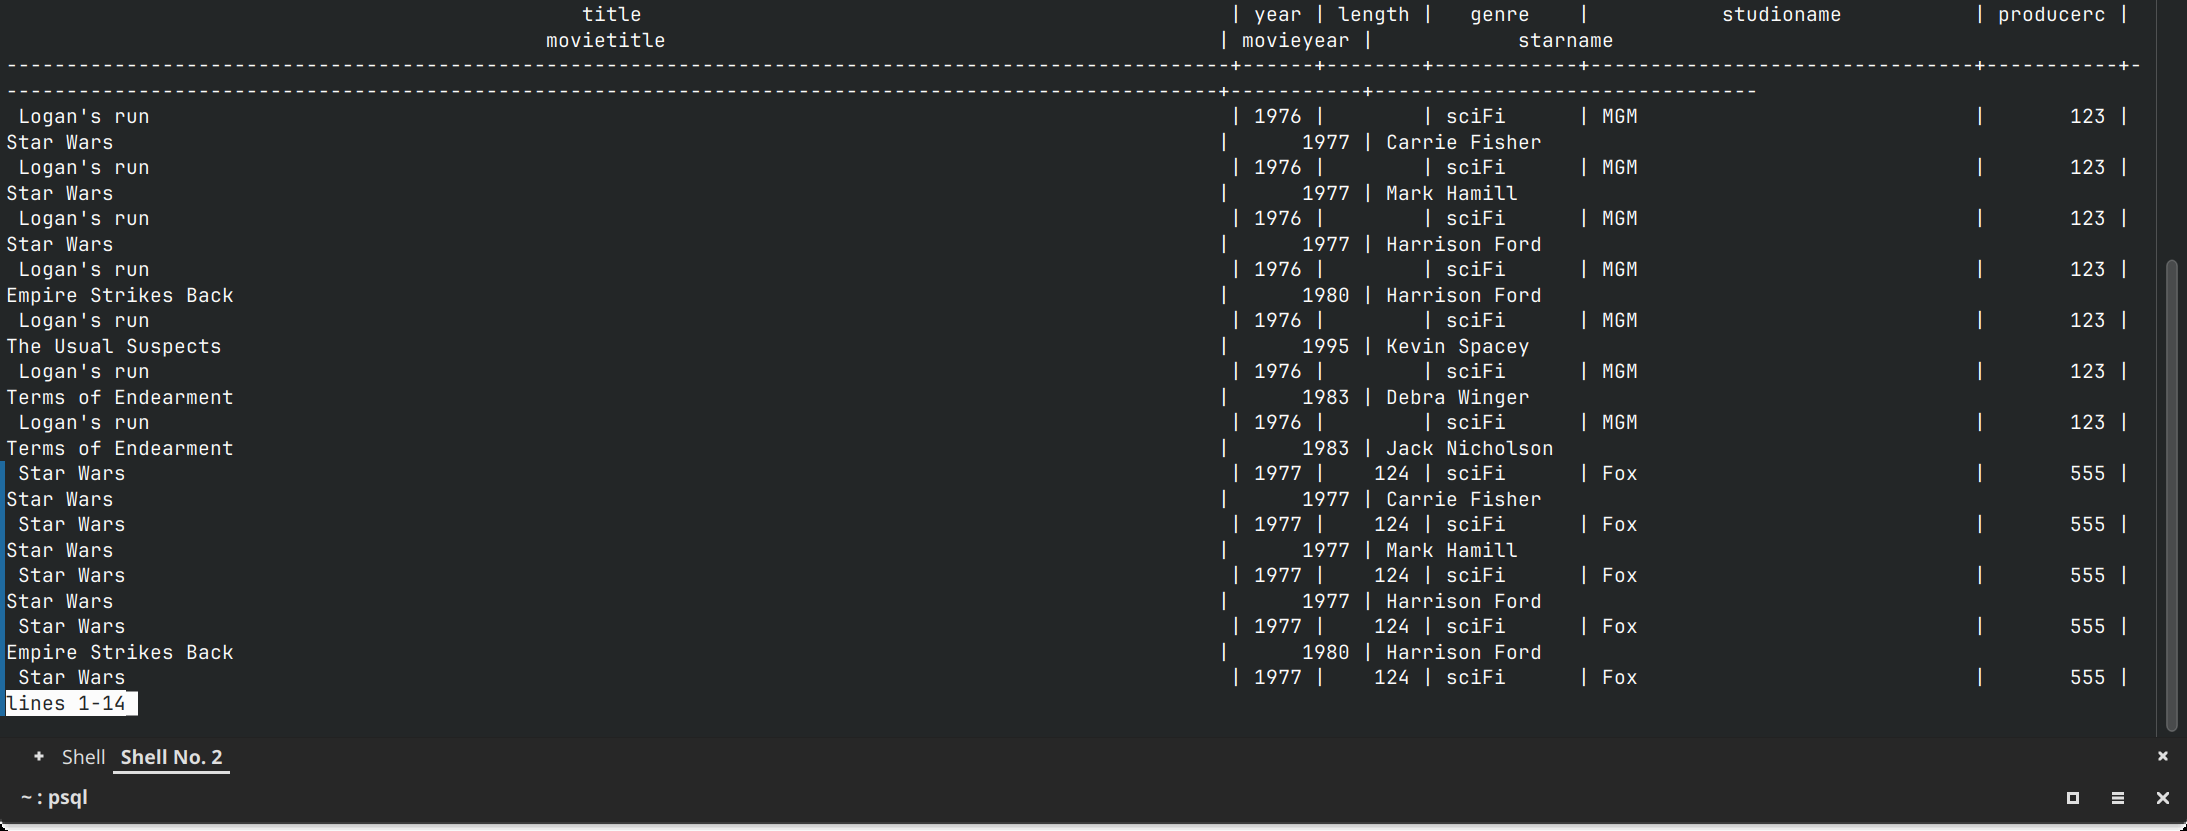
\includegraphics[width=0.8\textwidth]{hw5-12.png}
    \caption{Join Types}
    \label{fig:join-types-2}
\end{figure}

\begin{figure}[H]
    \centering
    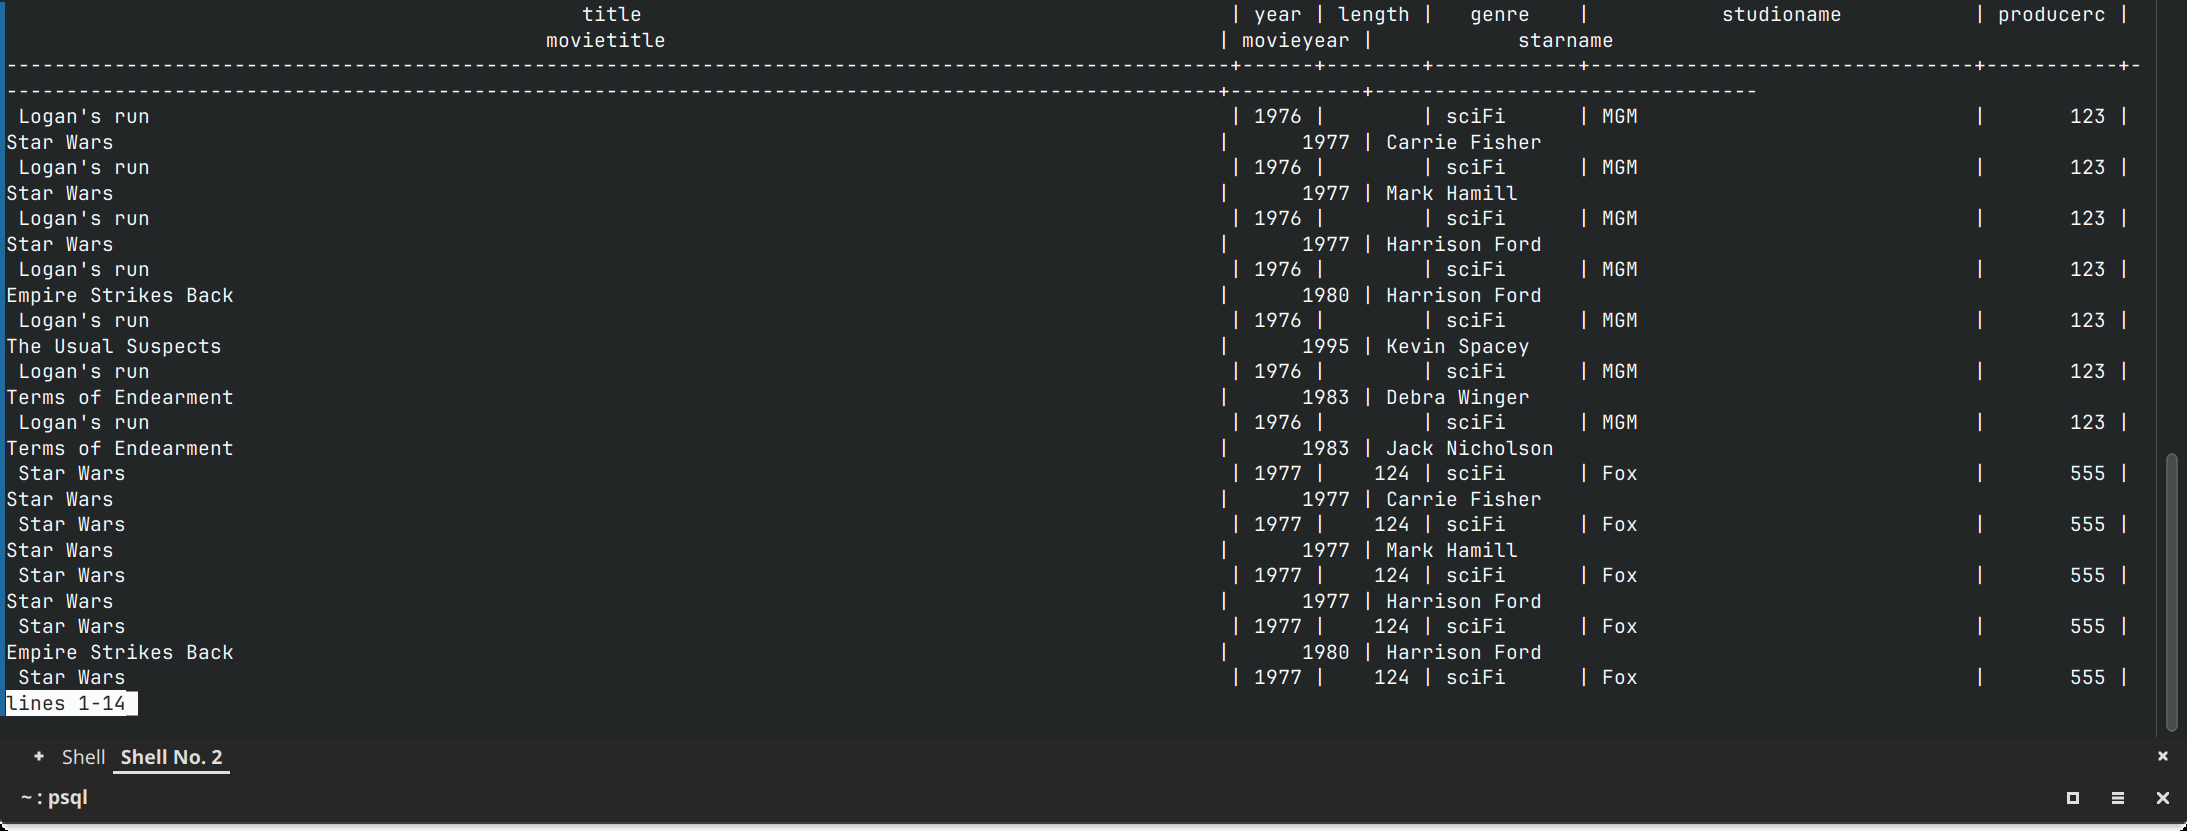
\includegraphics[width=0.8\textwidth]{hw5-13.png}
    \caption{Join Types}
    \label{fig:join-types-3}
\end{figure}

\begin{figure}[H]
    \centering
    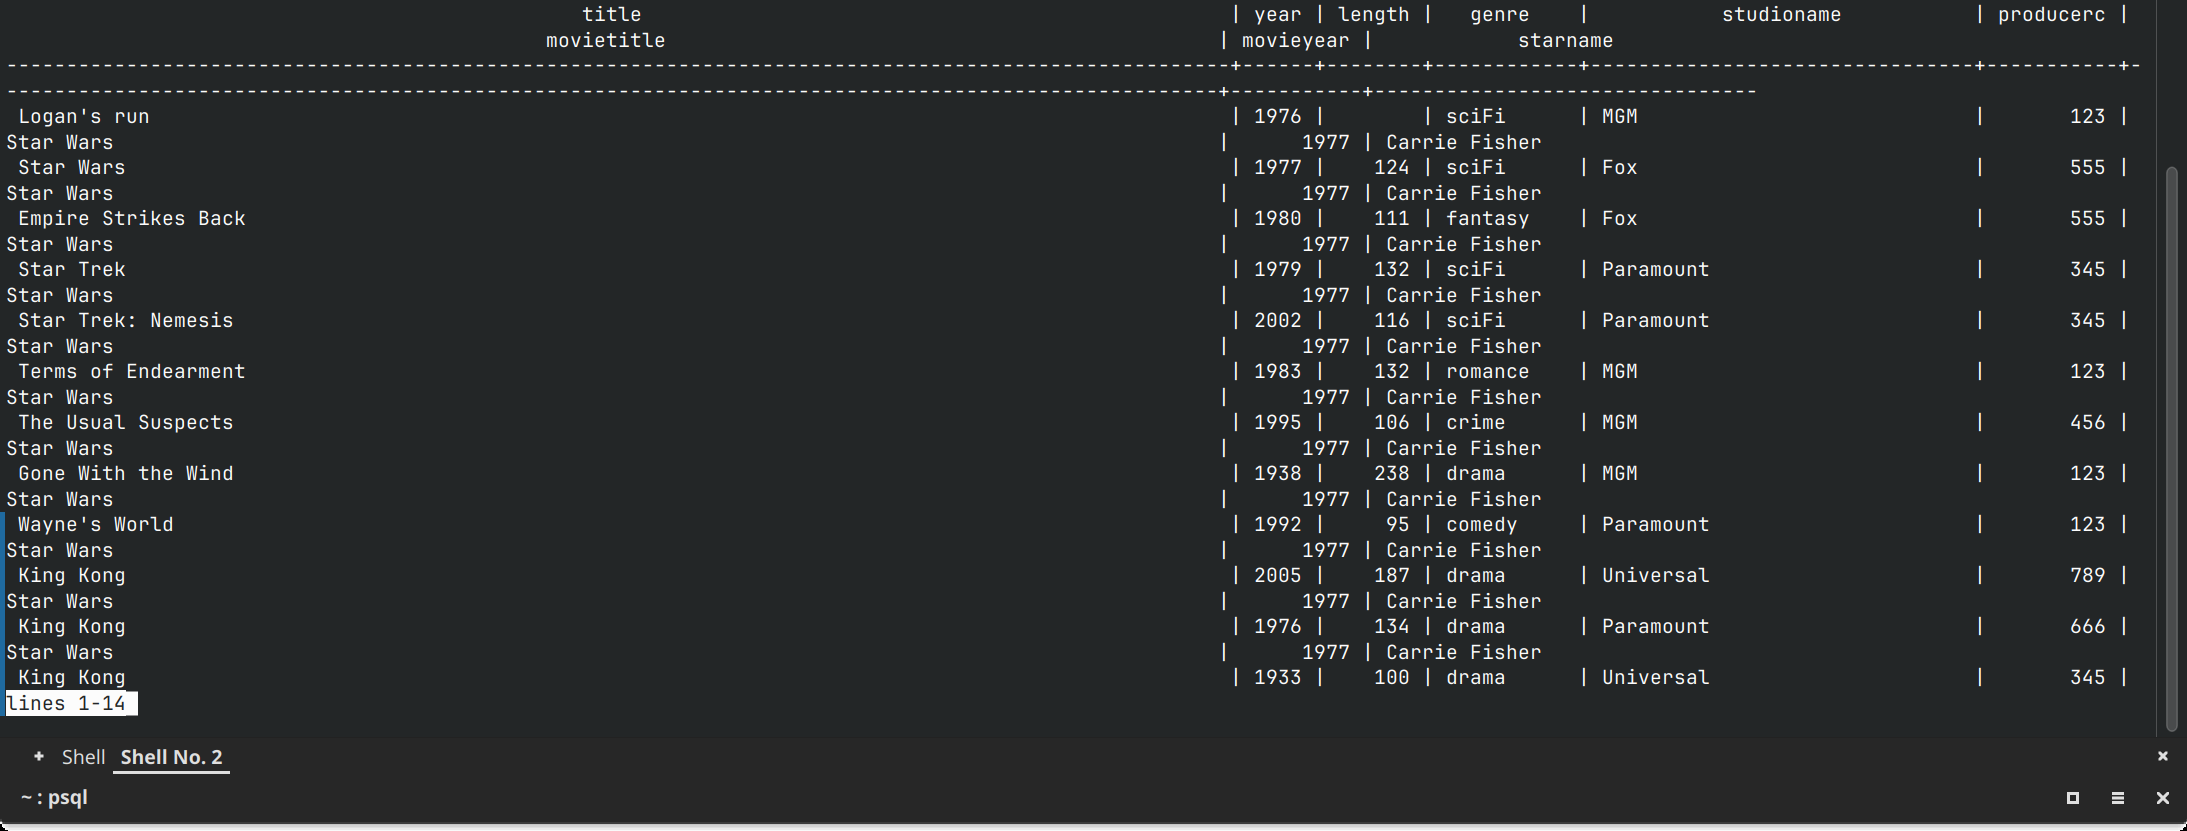
\includegraphics[width=0.8\textwidth]{hw5-14.png}
    \caption{Join Types}
    \label{fig:join-types-4}
\end{figure}

\subsubsection{Eliminating Duplicates}

\begin{lstlisting}[language=sql]
SELECT DISTINCT name
FROM MovieExec,
        Movies,
        StarsIn
WHERE cert = producerC
    AND title = movieTitle
    AND year = movieYear
    AND starName = 'Harrison Ford';
\end{lstlisting}

the execution results are shown in the Fig.~\ref{fig:eliminating-duplicates}.

\begin{figure}[H]
    \centering
    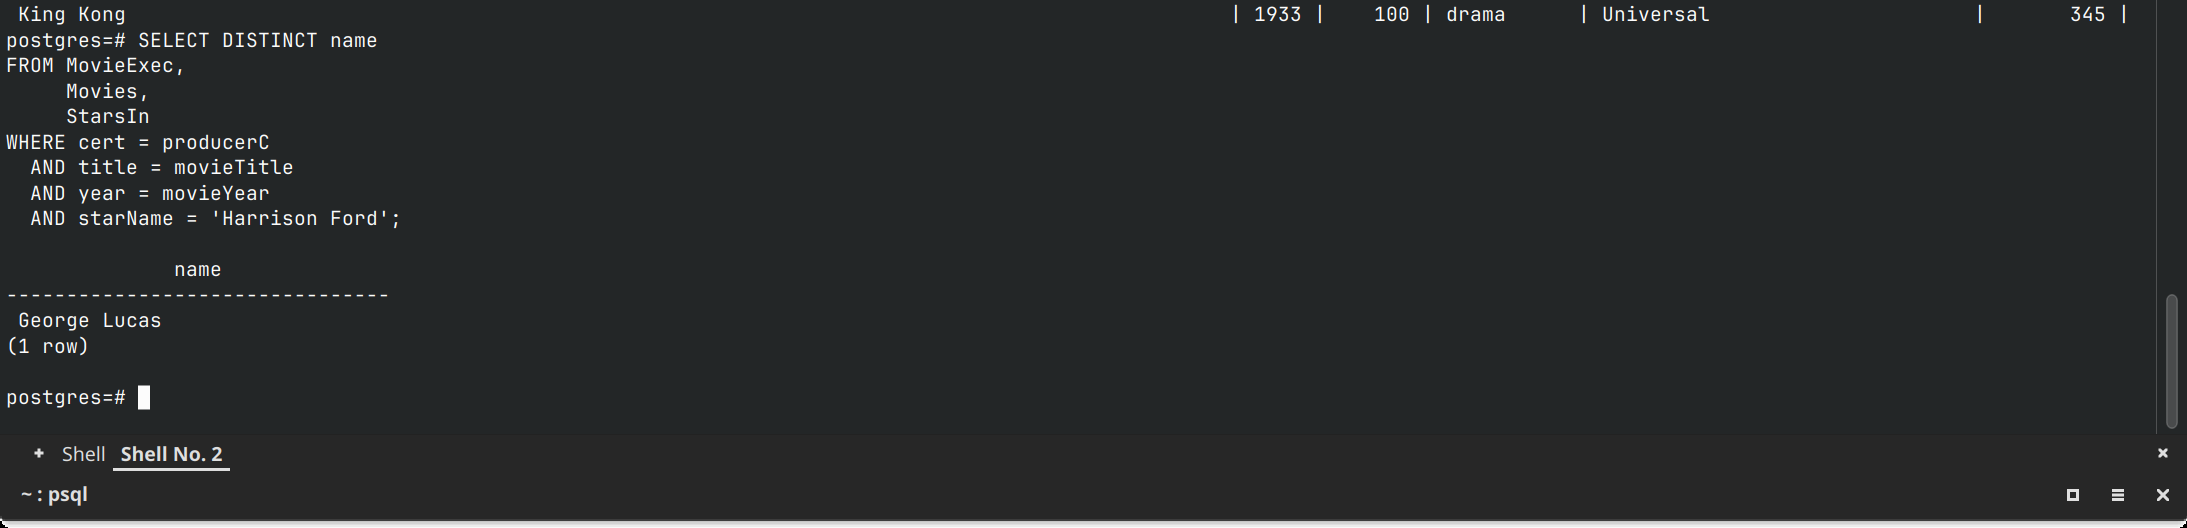
\includegraphics[width=0.8\textwidth]{hw5-15.png}
    \caption{Eliminating Duplicates}
    \label{fig:eliminating-duplicates}
\end{figure}


\subsubsection{Duplicates in Unions, Intersections, and Differences}

\begin{lstlisting}[language=sql]
(SELECT title, year FROM Movies)
UNION ALL
(SELECT movieTitle AS title, movieYear AS year FROM StarsIn);
\end{lstlisting}

the execution results are shown in the Fig.~\ref{fig:duplicates-in-unions}.
\begin{figure}[H]
    \centering
    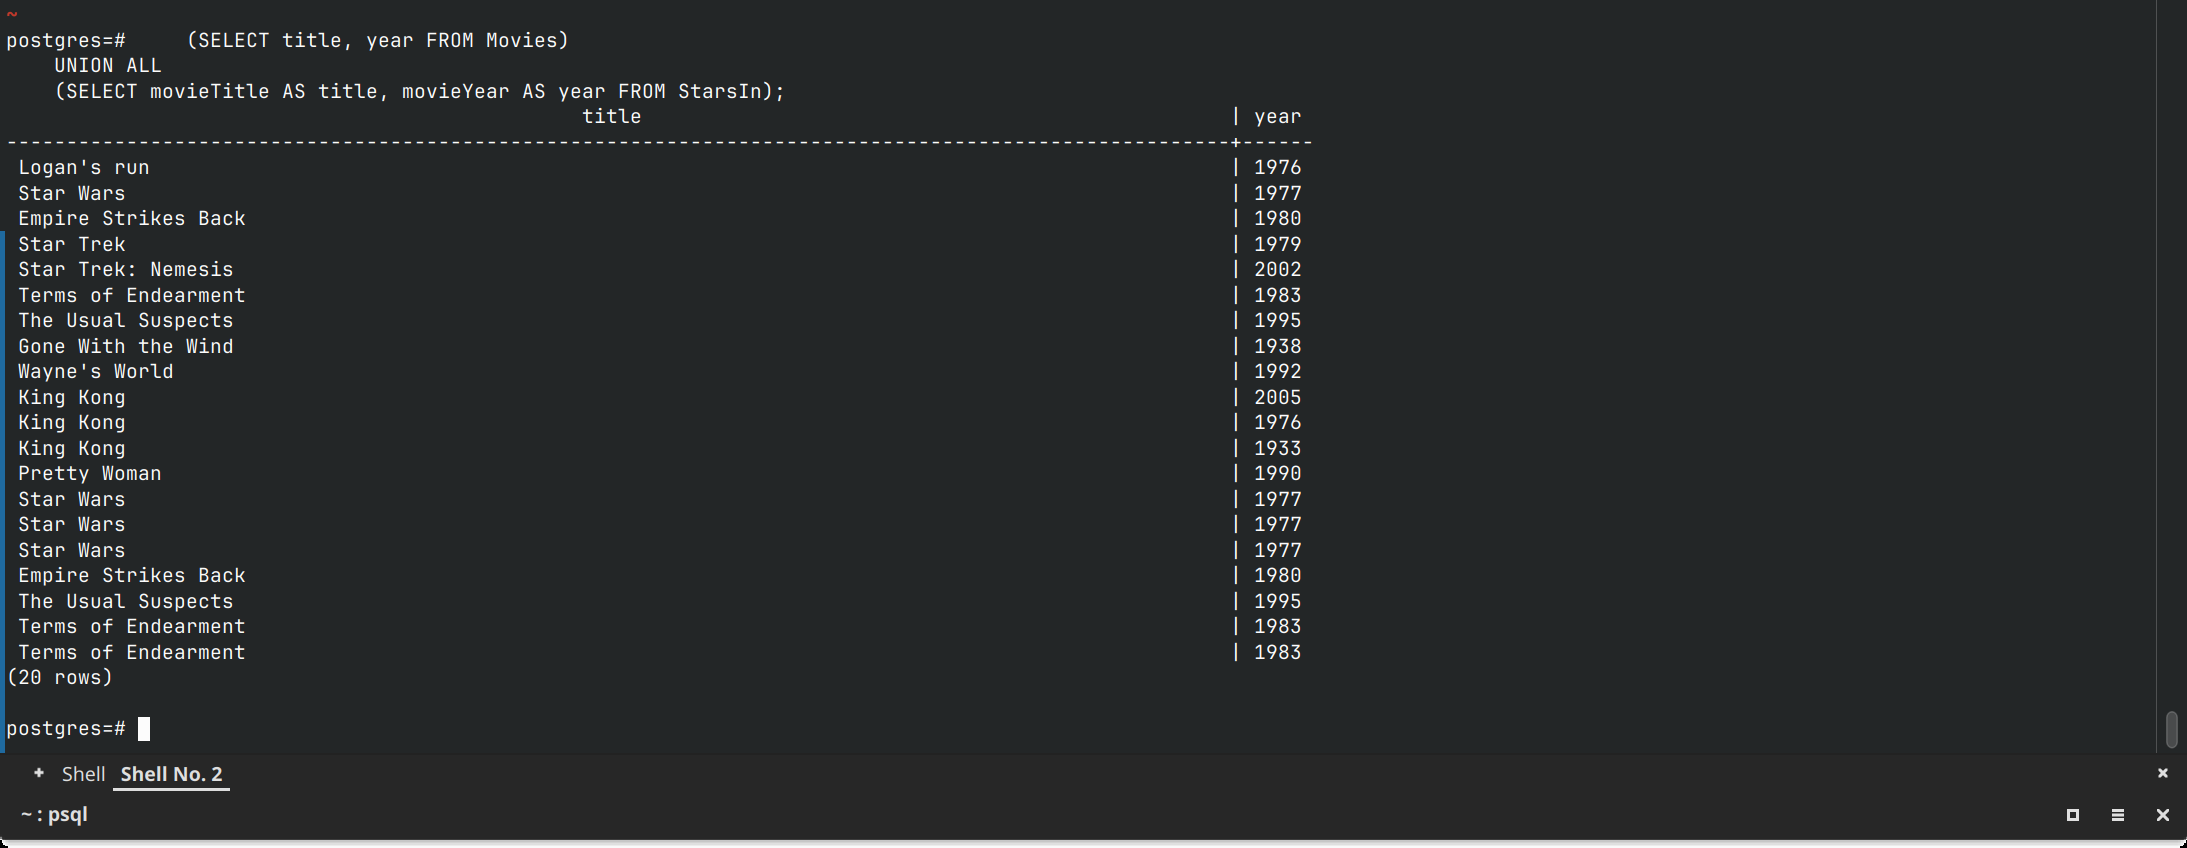
\includegraphics[width=0.8\textwidth]{hw5-16.png}
    \caption{Duplicates in Unions}
    \label{fig:duplicates-in-unions}
\end{figure}

\section{Excerise 6.3.2(a-d)}
Write the following queries, based on the database schema

\begin{itemize}
    \item Classes(class, type, country, numGuns, bore, displacement)
    \item Ships(name, class, launched)
    \item Battles(name, date)
    \item Outcomes(ship, battle, result)
\end{itemize}

You should use at least one subquery in each of your answers and write each query in two significantly different ways (e.g., using different sets of the operators EXISTS, IN, ALL, and ANY).

\begin{enumerate}
    \item[a)] Find the countries whose ships had the largest number of guns.
    \item[b)] Find the classes of ships, at least one of which was sunk in a battle.
    \item[c)] Find the names of the  ships with a 16-inch bore.
    \item[d)] Find the battles in which ships of the Kongo class participated.
\end{enumerate}

\subsection{Solutions}

\subsubsection*{a. Find the countries whose ships had the largest number of guns.}

\begin{lstlisting}[language=sql]
SELECT country
FROM Classes
WHERE numGuns = (SELECT MAX(numGuns) FROM Classes);
\end{lstlisting}

\subsubsection*{b. Find the classes of ships, at least one of which was sunk in a battle.}

\begin{lstlisting}[language=sql]
SELECT class
FROM Classes
WHERE class IN (
    SELECT class FROM Ships WHERE name IN (
        SELECT ship FROM Outcomes WHERE result = 'sunk'));
\end{lstlisting}

\subsubsection*{c. Find the names of the ships with a 16-inch bore.}

\begin{lstlisting}[language=sql]
SELECT name
FROM Ships
WHERE class IN (
    SELECT class FROM Classes WHERE bore = 16);
\end{lstlisting}

\subsubsection*{d. Find the battles in which ships of the Kongo class participated.}

\begin{lstlisting}[language=sql]
SELECT name
FROM Battles
WHERE name IN (
    SELECT battle FROM Outcomes WHERE ship IN (
        SELECT name FROM Ships WHERE class = 'Kongo'));
\end{lstlisting}

\section{Excerise 6.3.7}
For these relations from our running movie database schema

\begin{itemize}
    \item StarsIn(movieTitle, movieYear, starName)
    \item MovieStar(name, address, gender, birthdate)
    \item MovieExec(name, address, cert\#, netWorth)
    \item Studio(name, address, presC\#)
\end{itemize}

describe the tuples that would appear in the following SQL expressions:

\begin{enumerate}
    \item[a)] \texttt{Studio CROSS JOIN MovieExec;}
    \item[b)] \texttt{StarsIn NATURAL FULL OUTER JOIN MovieStar;}
    \item[c)] \texttt{StarsIn FULL OUTER JOIN MovieStar ON name = starName;}
\end{enumerate}

\subsection{Solutions}

\subsubsection*{a. \texttt{Studio CROSS JOIN MovieExec;}}

\begin{verbatim}
    (name, address, presC#, name, address, cert#, netWorth)
\end{verbatim}

\subsubsection*{b. \texttt{StarsIn NATURAL FULL OUTER JOIN MovieStar;}}

\begin{verbatim}
    (movieTitle, movieYear, starName, name, address, gender, birthdate)
\end{verbatim}

\subsubsection*{c. \texttt{StarsIn FULL OUTER JOIN MovieStar ON name = starName;}}
\begin{verbatim}
    (movieTitle, movieYear, starName, name, address, gender, birthdate)
\end{verbatim}


\section{Excerise 6.3.9}
Using the two relations

\begin{itemize}
    \item Classes(class, type, country, numGuns, bore, displacement)
    \item Ships(name, class, launched)
\end{itemize}

from our database schema of Exercise 2.4.3, write a SQL query that will produce all available information about ships, including that information available in the \texttt{Classes} relation. You need not produce information about classes if there are no ships of that class mentioned in \texttt{Ships}.

\subsection{Solutions}

\begin{lstlisting}[language=sql]
SELECT * FROM Ships
LEFT OUTER JOIN Classes ON Ships.class = Classes.class;
\end{lstlisting}

\end{document}